\chapter{模擬與評估系統表現}
\label{chp:4}


第三章中,我們建立了一個多LED對多PD系統的演算法,屬於定位流程中(參考圖\ref{pic:vlc_flow_draw})中Step4.值行定位演算法的步驟。而此演算法能夠在盡可能不限制Step1.決定次系統規格與Step2.系統設置的情況下,仍具有獲得三維定位以及目標物姿態的能力,不需限制觀察者與目標物平面平行,可廣用於不同使用情境上。此演算法在Step1.次系統規格的設置上保有許多自由度,包含選擇硬體規格、決定硬體數量$P,L$、設計硬體擺放的指向$\boldsymbol{V}$,因此本章節的主要目的便是探討Step1.中不同次系統規格對定位的影響。為了評估不同系統設計,我們首先需要利用硬體驗證或是軟體模擬的方法,完成完整的定位系統流程(參考圖\ref{pic:lp_system_flow}),以進行定位誤差的計算與評估。

\begin{figure}[htpb]
    \centering
    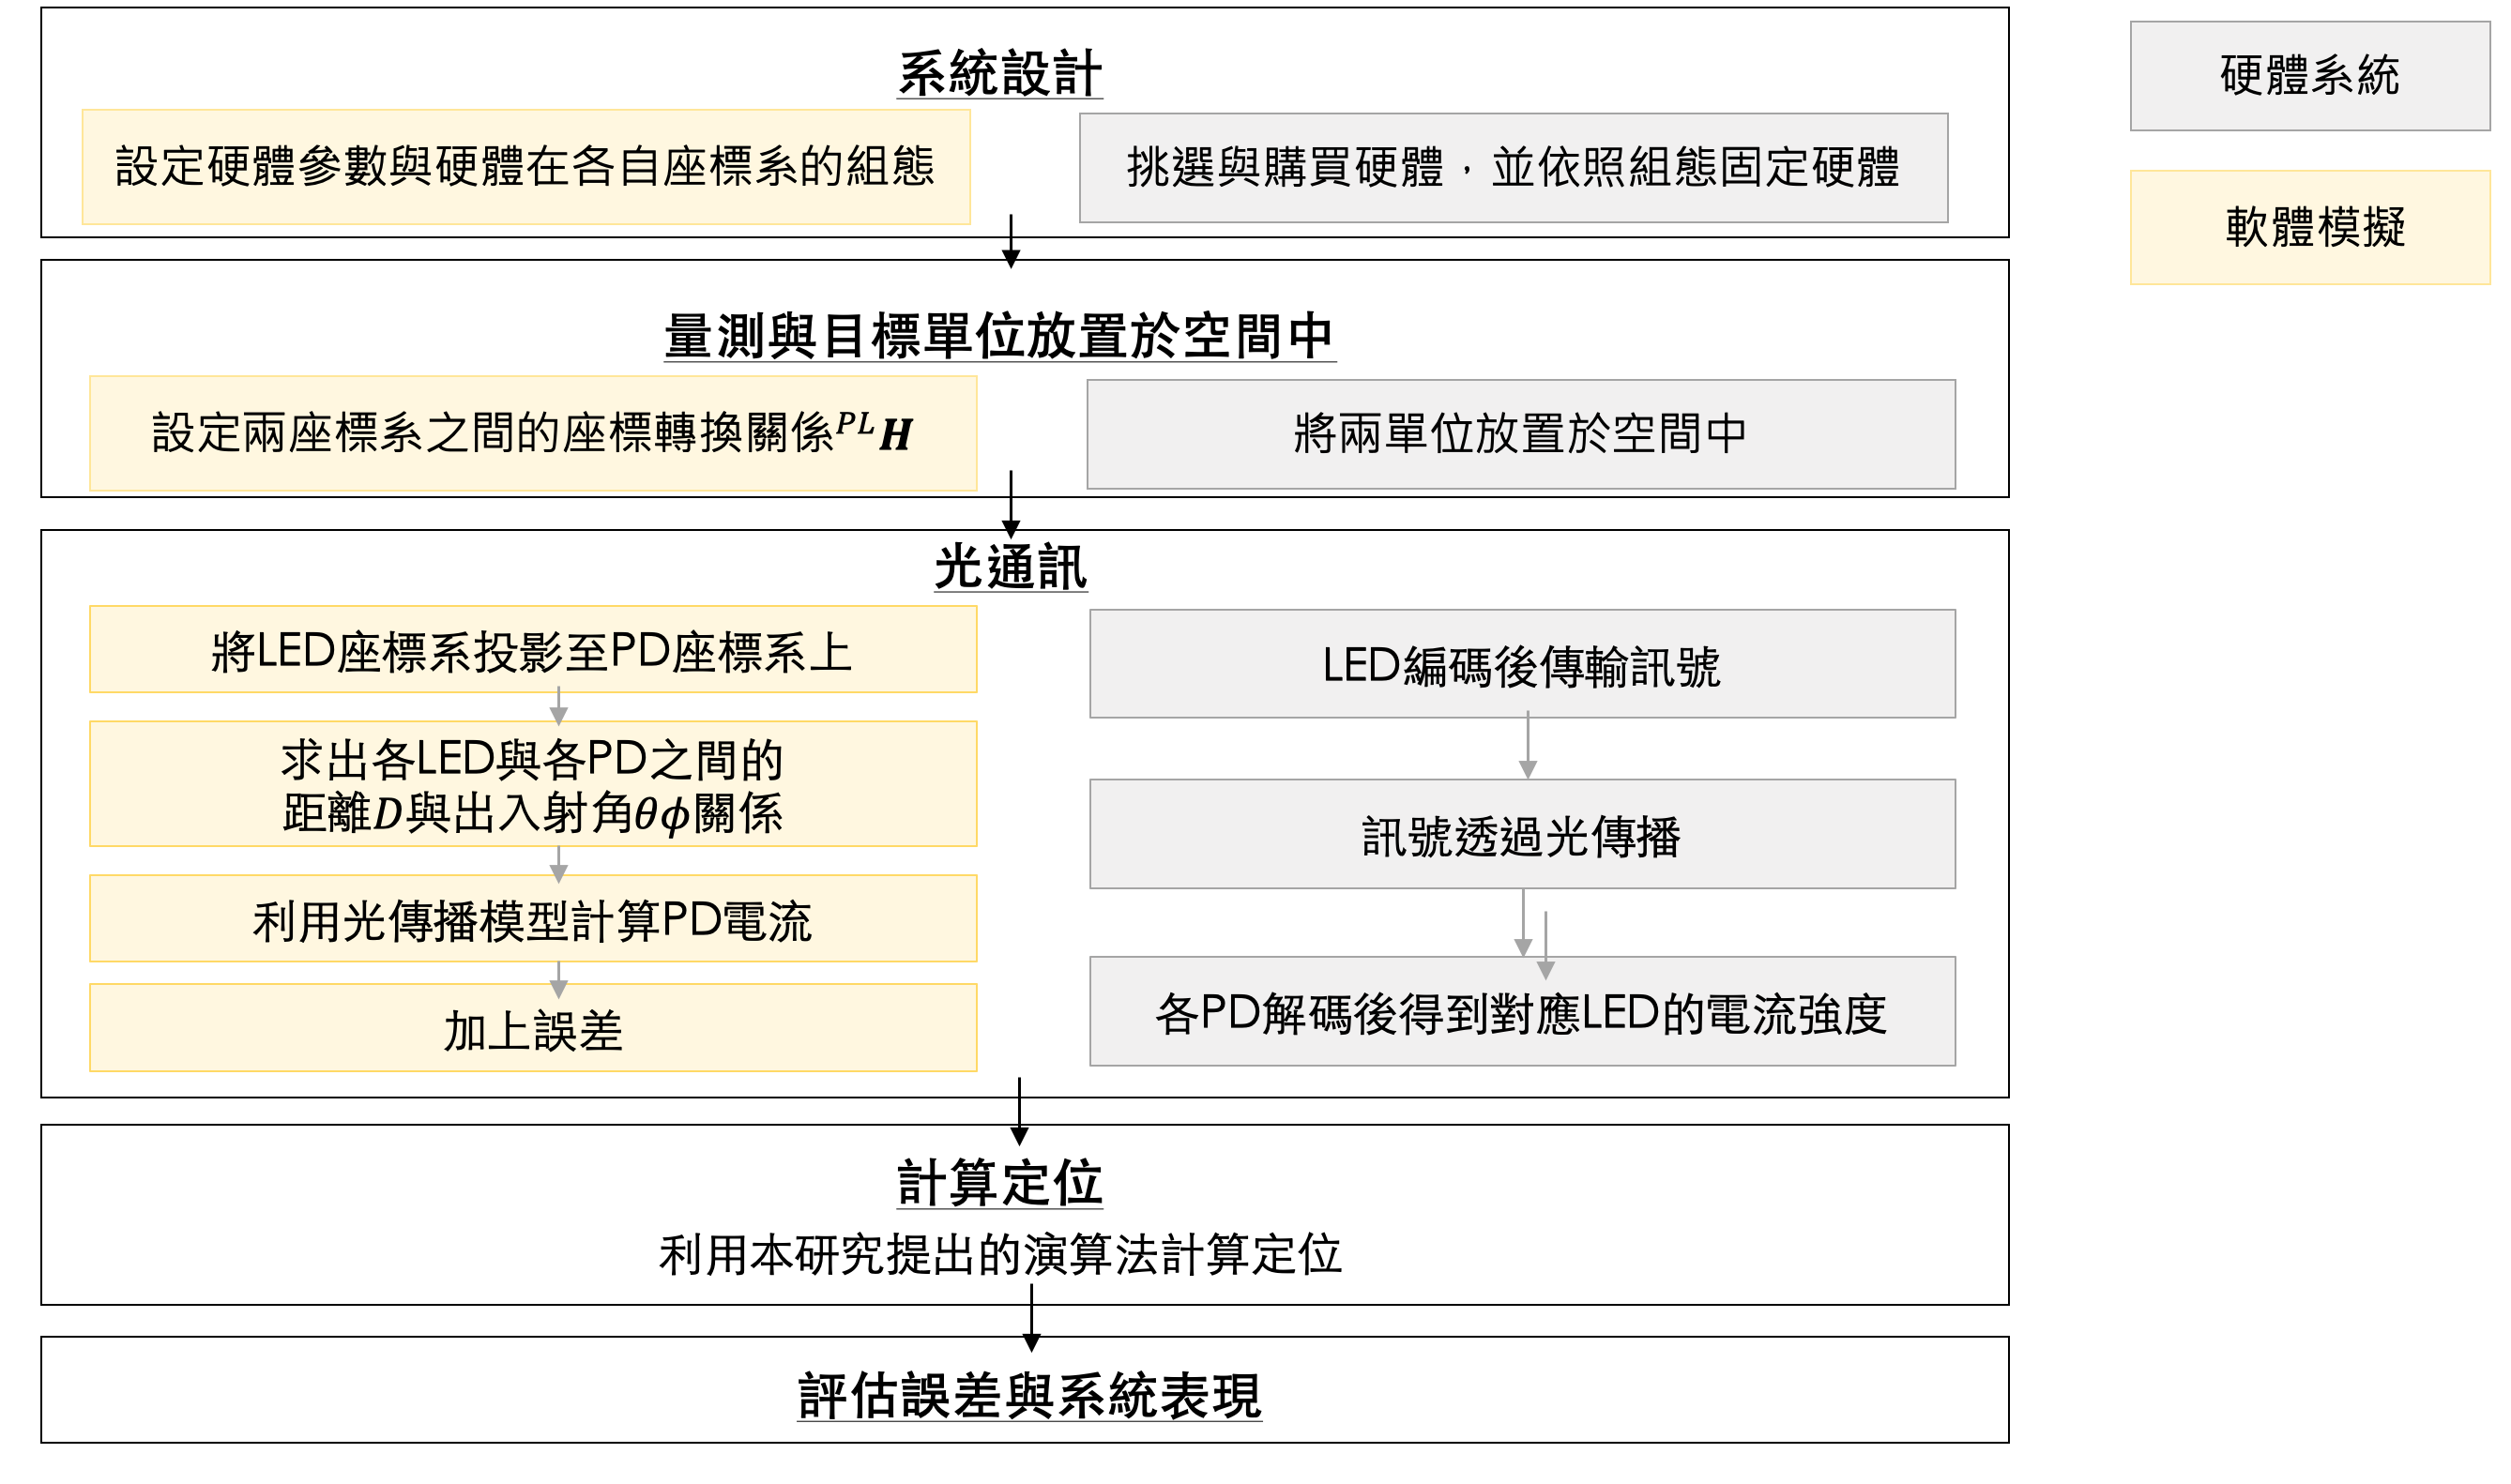
\includegraphics[width=15cm]{ch4pic/simulate_hardware.png}
    \caption{以硬體驗證與軟體模擬的流程圖}
    \label{pic:simulate_hardware}
\end{figure}

參考圖\ref{pic:simulate_hardware},硬體驗證的方法會由挑選硬體以及設計硬體模組開始,在完成次系統搭建後,將兩次系統的硬體單位放置於量測位置,透過光通訊的技術得到各LED對各PD的電流強度。軟體模擬的部分,則是以數學方式描述硬體參數、硬體擺法指向、以及兩座標系之間的轉換關係,並以光傳遞模型來模擬光通訊所得到的硬體輸出電流。比較硬體與軟體模擬的特性, 最完整的驗證方法為硬體驗證,然而由於光通訊發展並不如無線電波段成熟,架設光通訊系統較不方便,因此硬體驗證的複雜度較高;除此之外,硬體購買以及設計硬體模組的部分,都需要花費時間與金錢成本進行架設,在調整系統設計上也不如軟體靈活。也因此,大多數的文獻上會先透過軟體模擬,評估系統與演算法的表現,藉由低成本又快速方便的軟體模擬,在實際搭建硬體系統之前先對該設計有所了解,以做為硬體系統設計的參考。

因此,本論文會利用軟體模擬的方法,建立一模擬環境,將Step1.至Step3.的步驟在模擬中完成,再以第三章提出的定位演算法執行Step4.,各步驟如何以數學模型模擬實際情況與模擬中所需設定的參數於\ref{chp:simulation}章中詳細介紹。有了模擬方法後,我們於\ref{chp:simulate_result}章中設定一次系統規格並呈現其定位結果,並於\ref{chp:system_evaluate}章中則對不同的次系統規格設計進行效能評估,最後於\ref{chp:4_conclusion}章中總結。


\section{模擬方法}
\label{chp:simulation}

根據圖\ref{pic:simulate_hardware}中軟體模擬的流程,本章節由\ref{chp:system_design}章中介紹軟體模擬Step1.決定次系統規格中所需設定的參數,於\ref{chp:simulate_position}章中模擬Step2.系統設置兩硬體單位於不同位置的擺放,於\ref{chp:simulate_vlc}章中介紹模擬Step3.各PD接收到各LED的訊號的流程。




\subsection{模擬Step1.決定次系統規格}
\label{chp:system_design}

決定次系統規格時,我們需決定硬體數量$L,P$,以及硬體的規格與硬體的擺法$\boldsymbol{V}$,在此章節將敘述軟體模擬中需設定的數值,以及與與實際硬體系統設計時的差異。

\subsubsection{硬體數量}

決定硬體數量時,參考\ref{chp:orient_conclu}章中所述,LED與PD數量各需要最少三個來達成三維定位,因此在設定數量$L,P$時需確定其大於等於3,參考表\ref{tab:para_amount},兩參數為可自由設計的次系統設計變數。

\begin{table}[htpb]
    % \toprule% you can only use this within a tabular and if you load booktabs
    \renewcommand{\arraystretch}{1.3}
    \setlength{\arrayrulewidth}{0.15mm}
    \setlength{\doublerulesep}{0.12mm}
    \caption{模擬中需設定的硬體數量}
    \label{tab:para_amount}
    \centering
    \begin{tabular}{|cc|c|c|}
    \hline
    \multicolumn{2}{|c|}{\textbf{硬體數量}}  &\textbf{單位}  &  \textbf{備註}   \\
    \hline
     LED數量 &$L$ & 個 & 最小為3的整數 \\\hline
      PD數量& $P$& 個  & 最小為3的整數 \\\hline
    \end{tabular}
\end{table}
    
\subsubsection{硬體規格}

硬體規格在挑選時需著重注意的參數可以參考圖\ref{pic:hardware_para},包含影響輻射模式的朗博次方$Mp,M\ell$
,以及影響收發光強度的參數:LED總輻射通量$Pt$、PD有效面積$A$、飽和電流$s$、響應率$Re$;我們將這些參數統整於表\ref{tab:para_hardware}。這些參數中,除了朗博次方$M\ell,Mp$與有效面積$A$以外,各參數又會隨著給予的電壓電流改變。因此,\textbf{挑選朗博次方格外重要},一旦購買該規格硬體則無法調整輻射模型,不像其他可在購買後透過提高給定電壓電流來提升表現。

\begin{table}[htpb]
% \toprule% you can only use this within a tabular and if you load booktabs
\renewcommand{\arraystretch}{1.3}
\setlength{\arrayrulewidth}{0.15mm}
\setlength{\doublerulesep}{0.12mm}
\caption{模擬中需設定的硬體規格參數}
\label{tab:para_hardware}
\centering
\begin{tabular}{|c|cc|c|c|}
\hline
\multicolumn{3}{|c|}{\textbf{硬體參數}}  &\textbf{單位}  &  \textbf{備註}   \\
\hline
\multirow{2}{*}{LED} 
& 總輻射通量 &$Pt$ & $W$ & 可透過改變電壓調整 \\
 & 朗博次方& $M\ell$& -  & 最小為1 \\\hline
\multirow{4}{*}{PD} 
& 響應率 &$Re$ & $A/W$ & 可透過改變電壓調整 \\
& 有效面積& $A$& $m^2$ & - \\
& 飽和電流& $S$& $A$ & 可透過改變電壓調整 \\
& 朗博次方& $Mp$& -  & 最小為1 \\\hline
\end{tabular}
\end{table}

而在模擬中,所有參數皆可以透過簡單的調整數值來進行模擬;然而在現實中,一旦挑選了一種LED與PD,則硬體規格參數(表\ref{tab:para_hardware})與部分的誤差模擬參數數值基本上就被訂下。雖然仍能透過改變給定的電壓電流來調整硬體規格參數,但仍有一定的限制在,因此設定硬體參數的最佳方法,便是直接參考現有的硬體規格表,參考硬體規格表上的參數進行設定。因此,以下我們將現有市售的硬體規格列出,LED硬體規格呈現於表\ref{tab:para_LED}中,PD的硬體規格表中可參考的參數則呈現於表\ref{tab:para_PD}中,除了硬體規格參數以外也決定了後續\ref{chp:simulate_vlc}章節中的PD暗電流。

    \begin{table}[htpb]
        % \toprule% you can only use this within a tabular and if you load booktabs
        \renewcommand{\arraystretch}{1.3}
        \setlength{\arrayrulewidth}{0.15mm}
        \setlength{\doublerulesep}{0.12mm}
        \caption{市售的LED規格}
        \label{tab:para_LED}
        \centering
        \begin{tabular}{|cc|c|| c|c|c|}
        \hline
        \multicolumn{2}{|c|}{\textbf{參數}} & \textbf{單位}  
        & {Vishay}
        &{Hamamatsu}&
        Luxeon \\
        \multicolumn{2}{|c|}{} & {}  
        & {VSMA1085250\cite{datasheet:led_vsma}}
        &{L12170\cite{datasheet:hmL12170}} 
        & {L1IZ\cite{datasheet:led_luxeon}}\\
        \hline
        總輻射通量 &$Pt$ & $W$ & $5.34$ &$80\times 10^{-3}$ &1.15\\
        朗博次方& $M\ell$& -  & $5.57$ & $19.97$&1\\\hline
        % \multirow{4}{*}{PD} 
        % & 響應率 &$Re$ & $A/W$ & 可透過改變電壓調整 \\
        % & 有效面積& $A$& $m^2$ & - \\
        % & 飽和電流& $s$& $A$ & 可透過改變電壓調整 \\
        % & 朗博次方& $Mp$& -  & 最小為1 \\\hline
        \end{tabular}
    \end{table}
    
    \begin{table}[htpb]
            % \toprule% you can only use this within a tabular and if you load booktabs
            \renewcommand{\arraystretch}{1.3}
            \setlength{\arrayrulewidth}{0.15mm}
            \setlength{\doublerulesep}{0.12mm}
            \caption{市售的PD規格\cite{datasheet:hm_pd}}
            \label{tab:para_PD}
            \centering
            \begin{tabular}{|cc|c|| c|c|c|c|}
            \hline
            \multicolumn{2}{|c|}{\textbf{參數}} & \textbf{單位}  
            & {Hamamatsu}&{Hamamatsu} &{Hamamatsu} &{Hamamatsu}  \\
            \multicolumn{2}{|c|}{} & {}  
            & {S12915-16R}& {S12915-66R}& {S12915-1010R}& {S12698-02}
            \\
            \hline
            響應率 &$Re$ & $A/W$ & 0.64& 0.64& 0.64& 0.38 \\
            有效面積& $A$& $m^2$ & 
            $6\times 10^{-6}$ & 
            $3.3\times 10^{-5}$ & 
            $10^{-4}$ & 
            $3.36\times 10^{-5}$\\
            朗博次方& $Mp$& -  & $1$& $1$& $1$& $1.5$\\
            \hline
            % 分路電阻 &$Rs$ & $\Omega$ 
            % & $5\times 10^{10}$ 
            % & $10^{10}$
            % & $5\times 10^{9}$
            % & $10^{8}$  \\
            % 雜訊等效功率 &$Nep$ & $W/\sqrt{Hz}$ 
            % & $3.5\times 10^{-14}$ 
            % & $9\times 10^{-16}$
            % & $2\times 10^{-15}$
            % & $2.8\times 10^{-15}$\\
            PD暗電流 &$Id$ & $A$ 
            & $5\times 10^{-12}$ 
            & $5\times 10^{-11}$
            & $2\times 10^{-10}$
            & $10^{-10}$\\
            \hline
            \end{tabular}
    \end{table}
    

\subsubsection{硬體擺法}

硬體擺法的部分,位置的限制如\ref{chp:algorithm_constraint}章中所述,需限制PD擺放位置於PD座標系原點:$^P\boldsymbol{P}_p=
\left[\begin{array}{ccc}0&0&0\end{array}\right]^T$,LED的擺放位置也限制於LED座標系原點:$^L\boldsymbol{P}_l=
\left[\begin{array}{ccc}0&0&0\end{array}\right]^T$,而硬體擺放中的硬體指向$\boldsymbol{V}$則為可以自由設計之次系統設計變數。

而實際在設計硬體模組時,可以參考圖\ref{pic:ml_pd_config},需要將各電子元件與LED、PD硬體固定於一特殊形狀的載體上,利用其形狀來調整硬體的擺放指向。在模擬時,我們僅需透過定義各硬體的指向$\boldsymbol{V}$即可,其中各指向有兩個自由度:以球座標系定義的天頂角$\alpha$與方位角$\beta$。改變各硬體的指向時,各硬體的照射範圍也會改變,導致定位效果不同,因此硬體指向如何設計為一影響系統表現的因素,於\ref{chp:system_evaluate}章中進行評估。值得注意的是,每一個硬體的組態需要定義兩個自由度,因此擺法的部分,\textbf{總共需定義$2\times(L+P)$個自由度,硬體擺法的變數總數為硬體數量的函數},這個特性在後續第五章的最佳化問題中會使問題變十分複雜。

\begin{table}[htpb]
    % \toprule% you can only use this within a tabular and if you load booktabs
    \renewcommand{\arraystretch}{1.3}
    \setlength{\arrayrulewidth}{0.15mm}
    \setlength{\doublerulesep}{0.12mm}
    \caption{模擬中需設定的硬體組態}
    \label{tab:para_config}
    \centering
    \begin{tabular}{|c|cc|c|c|}
    \hline
    \multicolumn{3}{|c|}{\textbf{組態參數}}  &\textbf{單位}  &  \textbf{備註}   \\
    \hline
    \multirow{2}{*}{第$l$個LED} 
    & 天頂角 &$^L \alpha_l$ & $rad$ & $0\leq ^L \alpha_l<\pi$ \\
     & 方位角& $^L \beta_l$& $rad$ & $0\leq ^L \beta_l<2\pi$ \\\hline
    \multirow{2}{*}{第$p$個PD} 
    & 天頂角 &$^P \alpha_p$ & $rad$ & $0\leq ^P \alpha_p<\pi$ \\
    & 方位角& $^P \beta_p$& $rad$ & $0\leq ^P \beta_p<2\pi$ \\\hline
    \end{tabular}
    \end{table}

    

\subsection{模擬Step2.系統設置}
\label{chp:simulate_position}



根據\ref{chp:config}章中描述,LED與PD各自可視為一個座標系,而兩者之間的相對關係可以齊次座標轉換表示,參考\ref{chp:relative}章。因此,我們可以透過改變齊次轉換矩陣$^{PL}\boldsymbol{H}$,使兩座標系之間的相對關係改變,以模擬兩硬體單位於空間中擺放位置。

而根據式\ref{eqn:homogeneous}中呈現,齊次座標轉換矩陣$^{PL}\boldsymbol{H}$可以視為平移向量$^{PL}\boldsymbol{T}$與旋轉矩陣$^{PL}\boldsymbol{Ro}$綜合的效果,而平移與旋轉各自三個自由度,呈現於表\ref{tab:para_relative}。我們透過定義平移矩陣與旋轉矩陣來模擬兩硬體單位於空間中的相對位置,如式\ref{eqn:simulate_position},平移位置透過$^{PL}t_x,^{PL}t_y,^{PL}t_z$三項定義,而旋轉則透過翻滾角$^{PL}rx$(Roll)、俯仰角$^{PL}ry$(Pitch)、偏航角$^{PL}rz$(Yaw)定義,各自代表繞x,y,z軸旋轉的角度,則旋轉矩陣可以寫為$^{PL}\boldsymbol{Rx},^{PL}\boldsymbol{Ry},^{PL}\boldsymbol{Rz}$三個矩陣的相乘結果。

\begin{equation}
    \label{eqn:simulate_position}
    \begin{aligned}
    ^{PL}\boldsymbol{T} &= 
    \left[\begin{array}{c}
        ^{PL}t_x \\^{PL}t_y\\^{PL}t_z
    \end{array}\right]\\
    ^{PL}\boldsymbol{Ro} &= 
    ^{PL}\boldsymbol{Rz} (^{PL}rz)^{PL}\boldsymbol{Ry}(^{PL}ry) ^{PL}\boldsymbol{Rx} (^{PL}rx)\\
    \text{Where }&\\
    &^{PL}\boldsymbol{Rx} (^{PL}rx) =
    \left[ \begin{array}{ccc}
        1&0&0\\
        0&\cos (^{PL}rx) &-\sin (^{PL}rx) \\
        0&\sin (^{PL}rx) &\cos (^{PL}rx) 
    \end{array}\right] \\
    &^{PL}\boldsymbol{Ry}(^{PL}ry)=
    \left[ \begin{array}{ccc}
        \cos (^{PL}ry) &0&\sin (^{PL}ry) \\
        0&1&0\\
        -\sin (^{PL}ry) &0&\cos (^{PL}ry)
    \end{array}\right]\\
    &^{PL}\boldsymbol{Rz} (^{PL}rz) = 
    \left[ \begin{array}{ccc}
        \cos (^{PL}rz) &-\sin (^{PL}rz)& 0 \\
        \sin (^{PL}rz) &\cos (^{PL}rz)& 0 \\
        0 &0&1
    \end{array}\right]\\
    \end{aligned}
\end{equation}

\begin{table}[htpb]
    % \toprule% you can only use this within a tabular and if you load booktabs
    \renewcommand{\arraystretch}{1.3}
    \setlength{\arrayrulewidth}{0.15mm}
    \setlength{\doublerulesep}{0.12mm}
    \caption{模擬中定義相對位置的參數}
    \label{tab:para_relative}
    \centering
    \begin{tabular}{|c|cc|c|c|}
    \hline
    \multicolumn{3}{|c|}{\textbf{定義相對位置的參數}}  &\textbf{單位}  &  \textbf{備註}   \\
    \hline
    \multirow{3}{*}{平移向量$^{PL}\boldsymbol{T}$自由度} 
    & x分量 &$^{PL}t_x$ & $m$ &  \\
    & y分量 &$^{PL}t_y$ & $m$ &  \\
    & z分量 &$^{PL}t_z$ & $m$ &  \\
    \hline
    \multirow{3}{*}{旋轉矩陣$^{PL}\boldsymbol{Ro}$自由度} 
    & Roll &${^{PL}rx}$ & $rad$ &  $0\leq {^{PL}rx}<2\pi$\\
    & Pitch &$^{PL}ry$ & $rad$ & $0\leq {^{PL}rx}<2\pi$ \\
    & Yaw &$^{PL}rz$ & $rad$ & $0\leq {^{PL}rx}<2\pi$ \\
    \hline
    \end{tabular}
    \end{table}

    而由於本論文使用的演算法並沒有對Step2.系統設置進行限制,因此表\ref{tab:para_relative}中的參數可以任意設置,使兩次系統座標系根據使用情境,於感興趣空間中(Region of Interest,以下簡稱ROI)自由移動。

\subsection{模擬Step3.LED發送與PD接收訊號}
\label{chp:simulate_vlc}

    \begin{figure}[htpb]
        \centering
        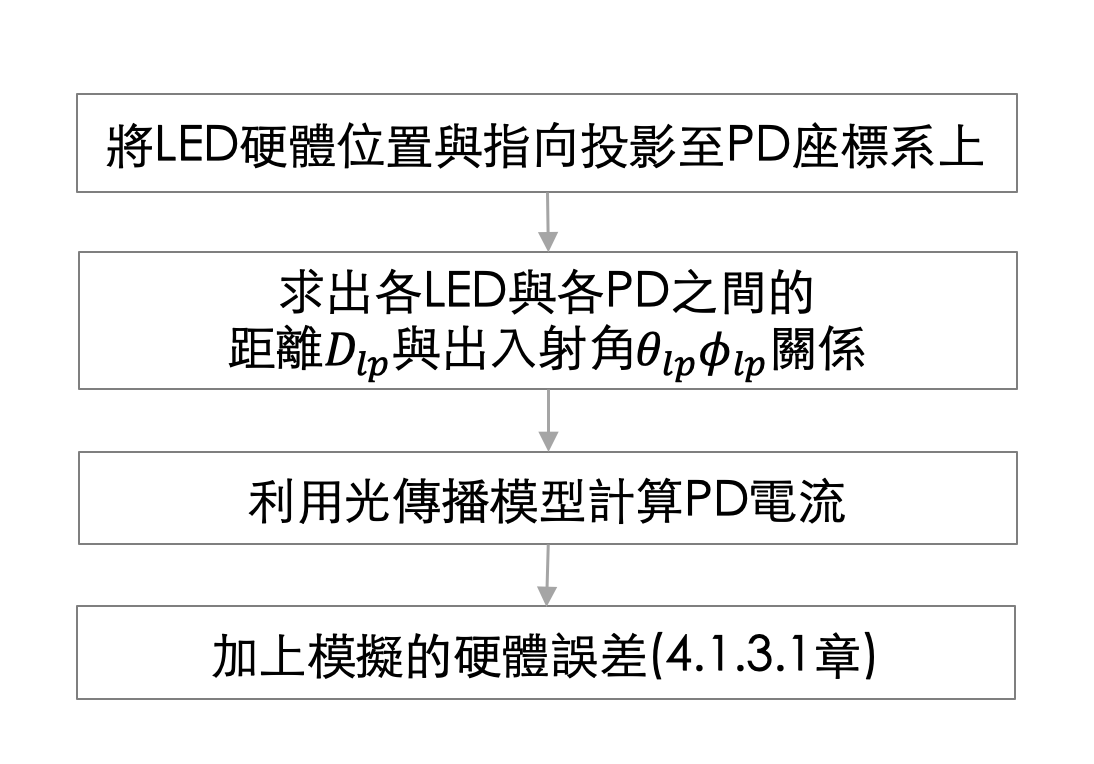
\includegraphics[width=10cm]{ch4pic/simulate_signal_flow.png}
        \caption{模擬Step3.LED發送與PD接收訊號之流程圖}
        \label{pic:simulate_signal_flow}
    \end{figure}

    模擬Step3.LED發送與PD接收訊號的步驟參考圖\ref{pic:simulate_signal_flow},將LED硬體位置與指向投影至PD座標系上後,於PD座標系中求出各LED與PD之間的距離$D_{lp}$與出入射角$\phi_{lp},\theta_{lp}$的關係,由此套入光傳播模型計算PD電流。以上這三個步驟與\ref{chp:model}中以次系統座標系表達光傳遞模型的步驟相同,可以透過式\ref{eqn:model_coor_extend}描述如何利用硬體規格參數、硬體擺法、兩次系統相對關係,計算出理論的PD電流輸出$Ie_{lp}$。然而實際情況下,硬體量測具有誤差,因此我們參考大多文獻模擬誤差的方式,於\ref{chp:hardware_error}章中介紹。

    \subsubsection{模擬硬體誤差}
    \label{chp:hardware_error}

    圖\ref{pic:simulate_hardware}流程中,模擬光通訊的部分可透過式\ref{eqn:model_algorithm_filter}獲得理論的PD電流強度,而為了更真實的模擬現實狀況,參考\cite{survey_light2018}中對誤差的模擬,呈現於式\ref{eqn:noise}中:$\hat{Ie}_{lp}$代表第l個LED對第p個PD模擬出的硬體輸出電流,其組成包含了理論的量測電流$Ie_{lp}$與PD硬體誤差$In$。其中,PD硬體誤差中,又可分為熱雜訊$It$(Thermal Noise)與散粒雜訊$Is$(Shot Noise),兩者皆可以用常態分佈(Normal Distribution)描述,因此各自以$It^2$與$Is^2$表示雜訊的變異數(Varaiance),呈現於式\ref{eqn:thermal_noise}與式\ref{eqn:shot_noise}中,其中$Kb$為波茲曼常數(Boltzmann constant)、$Te$為絕對溫度、$B$為頻寬、$R$為感測電路的電阻、$q$為電子電荷、$Ib$為背景電流、$Id$為PD暗電流。

    \begin{equation}
    \label{eqn:noise}
        \hat{Ie}_{lp}=Ie_{lp}+In 
    \end{equation}


    \begin{gather}
        \label{eqn:thermal_noise}
        In^2 = {It_{lp}^2+Is_{lp}^2}
        It_{lp}^2={\frac{4 Kb Te B}{R}}\\
        \label{eqn:shot_noise}
        Is_{lp}^2={2q(Ie_{lp}+Ib+Id)B}
    \end{gather}

    % 除了加上誤差以外,我還需評估硬體的解析度,光電二極體的解析度,也就是PD最小可感測的電流$Im$,可以用雜訊等效功率$Nep$(noise equivalent power,以下簡稱NEP)計算,如式\ref{eqn:nep},,而NEP大小則取自硬體規格表。

    % \begin{gather}
    %     \label{eqn:nep}
    %     Im = Nep\times \sqrt{B}
    % \end{gather}

    我們將模擬硬體誤差所需設定的參數整理於表\ref{tab:para_error}:

    \begin{table}[htpb]
        % \toprule% you can only use this within a tabular and if you load booktabs
        \renewcommand{\arraystretch}{1.3}
        \setlength{\arrayrulewidth}{0.15mm}
        \setlength{\doublerulesep}{0.12mm}
        \caption{模擬硬體誤差需定義的參數}
        \label{tab:para_error}
        \centering
        \begin{tabular}{|cc|c|c|}
        \hline
        \multicolumn{2}{|c|}{\textbf{模擬硬體誤差的參數}}  &\textbf{單位}  &  \textbf{備註}   \\
        \hline
        絕對溫度 &$Te$ & $K$ &  \\
        頻寬 &$B$ & $Hz$ &  \\
        電阻 &$R$ & $\Omega$ &  \\
        % 雜訊等效功率 &$Nep$ & $W/\sqrt{Hz}$ &  \\
        PD暗電流 &$Id$ & $A$ &  \\
        背景電流 &$Ib$ & $A$ &  \\
        \hline
        \end{tabular}
    \end{table}


    表\ref{tab:para_error}的參數中,PD暗電流如\ref{chp:para_hardware}可以參考硬體規格表\ref{tab:para_PD}設定,而其餘參數則需依照使用情境進行調整。絕對溫度我們取$300K$作為室內溫度,而頻寬與背景電流則選擇參考其他文獻來決定參數,這邊選擇參考文獻\cite{omg_old},數值呈現於表\ref{tab:para_from_cite}。


    \begin{table}[h!]
        % \toprule% you can only use this within a tabular and if you load booktabs
        \renewcommand{\arraystretch}{1.3}
        \setlength{\arrayrulewidth}{0.15mm}
        \setlength{\doublerulesep}{0.12mm}
        \caption{參考其他文獻之參數數值}
        \label{tab:para_from_cite}
        \centering
        \begin{tabular}{|cc|c|c|}
        \hline
        \multicolumn{2}{|c|}{\textbf{模擬硬體誤差的參數}}  &\textbf{單位}  &  \textbf{數值}   \\
        \hline
        絕對溫度 &$Te$ & $K$ &  $300$\cite{omg_old} \\
        頻寬 &$B$ & $Hz$ &  $640\times 10^{3}$ \cite{omg_old}\\
        背景電流 &$Ib$ & $A$ &  $740\times 10^{-6}$ \cite{omg_old}\\
        \hline
        \end{tabular}
    \end{table}










\section{呈現定位結果}
\label{chp:simulate_result}

上一章節中,我們介紹了如何利用軟體模擬的方式,模擬LED與PD定位系統的Step1.決定次系統規格、Step2.系統設置、Step3.LED發送與PD接收訊號,並設定各模擬參數;在此章節,我們則要利用此模擬方法,將次系統規格帶入模型中進行定位,得到兩硬體於空間中各位置計算出的定位$\hat{^{PL}\boldsymbol{T}}$,而定位誤差則定義為其與定義相對位置的平移向量$^{PL}\boldsymbol{T}$之間的歐氏距離,參考式\ref{eqn:error_dis}。


\begin{equation}
    \label{eqn:error_dis}
    \hat{e} = ||\hat{^{PL}\boldsymbol{T}}-^{PL}\boldsymbol{T}||
\end{equation}

% 本章節將於\ref{chp:simulate_para}章中紀錄如何抉擇模擬中Step1.至Step3.所需使用的參數,而經過Step4.執行定位演算法後的結果則呈現於\ref{chp:simulate_result_sub}章中。


% \subsection{設定模擬所需參數}
% \label{chp:simulate_para}

% 在此段落,我們介紹如何設定\ref{chp:simulation}章中須設置的參數們,包含Step1.次系統規格中的硬體數量(表\ref{tab:para_amount})、硬體參數(表\ref{tab:para_hardware})、硬體組態(表\ref{tab:para_config}),與Step2.系統設置中的座標系相對關係(表\ref{tab:para_relative}),還有Step3.LED發送與PD接收訊號的誤差模擬參數(表\ref{tab:para_error})。因此我們將\ref{chp:simulation}章中提到需要設定的參數們,依照參數設定參考的方式分為三類,\ref{chp:para_hardware}章中介紹參考市售硬體規格表決定的參數,\ref{chp:para_from_cite}章中則參考文獻決定部分參數,其餘則為Step1.次系統規格與Step2.系統設置中可以自由設計的系統設計變數,於\ref{chp:para_can_design}章中介紹。



% \subsubsection{參考市售硬體規格表設定之參數}
% \label{chp:para_hardware}




% \subsubsection{參考其他文獻設定之參數}
% \label{chp:para_from_cite}



% \subsubsection{可自由設計之參數}
% \label{chp:para_can_design}

% 除了以上參數以外,硬體數量(表\ref{tab:para_amount})、硬體擺法的指向$\boldsymbol{V}$(表\ref{tab:para_config})為可自由設計的Step1.次系統規格設計變數,而Step2.中系統設置描述坐標系相對關係(表\ref{tab:para_relative})則會依照不同的使用情境而改變。

% 為描述相對位置與情境方法。



% \subsection{模擬結果}
% \label{chp:simulate_result_sub}

因此,我們建立了一個互動模擬介面如圖\ref{pic:result_interactive},硬體規格參數選用表\ref{tab:para_LED}中的Luxeon L1IZ與表\ref{tab:para_PD}中的Hamamatsu S12915-1010R兩者的參數,而誤差模擬參數則以表\ref{tab:para_from_cite}的參數帶入。在這個模擬介面中,我們可以透過改變自由設計的系統設計變數、兩次系統之間的相對位置、以及一些硬體與電路參數,來觀察定位的效果。其中,硬體指向的部分,由於每個硬體都有兩個自由度,為了方便進行模擬,這裡將指向暫時限制成文獻中最常見的樣式,也就是$^P\boldsymbol{V}_p^{sph}$中的方位角平均分配:$^P\beta_p = 1\pi/P$,而各PD的天頂角則限制為相同:$^P\alpha_p =^P \alpha$,因此PD唯一的擺法自由度剩下$^P\alpha$天頂角,參考圖\ref{pic:config_orient}。

% 根據\ref{chp:simulation}章所述系統設計與誤差模擬方法,模擬參數初始值則選用,其餘誤差模擬參數以表\ref{tab:para_from_cite}的參數帶入,則可以透過調整各項參數、座標系相對關係來看定位結果與定位誤差。


\begin{figure}[htpb]
    \centering
    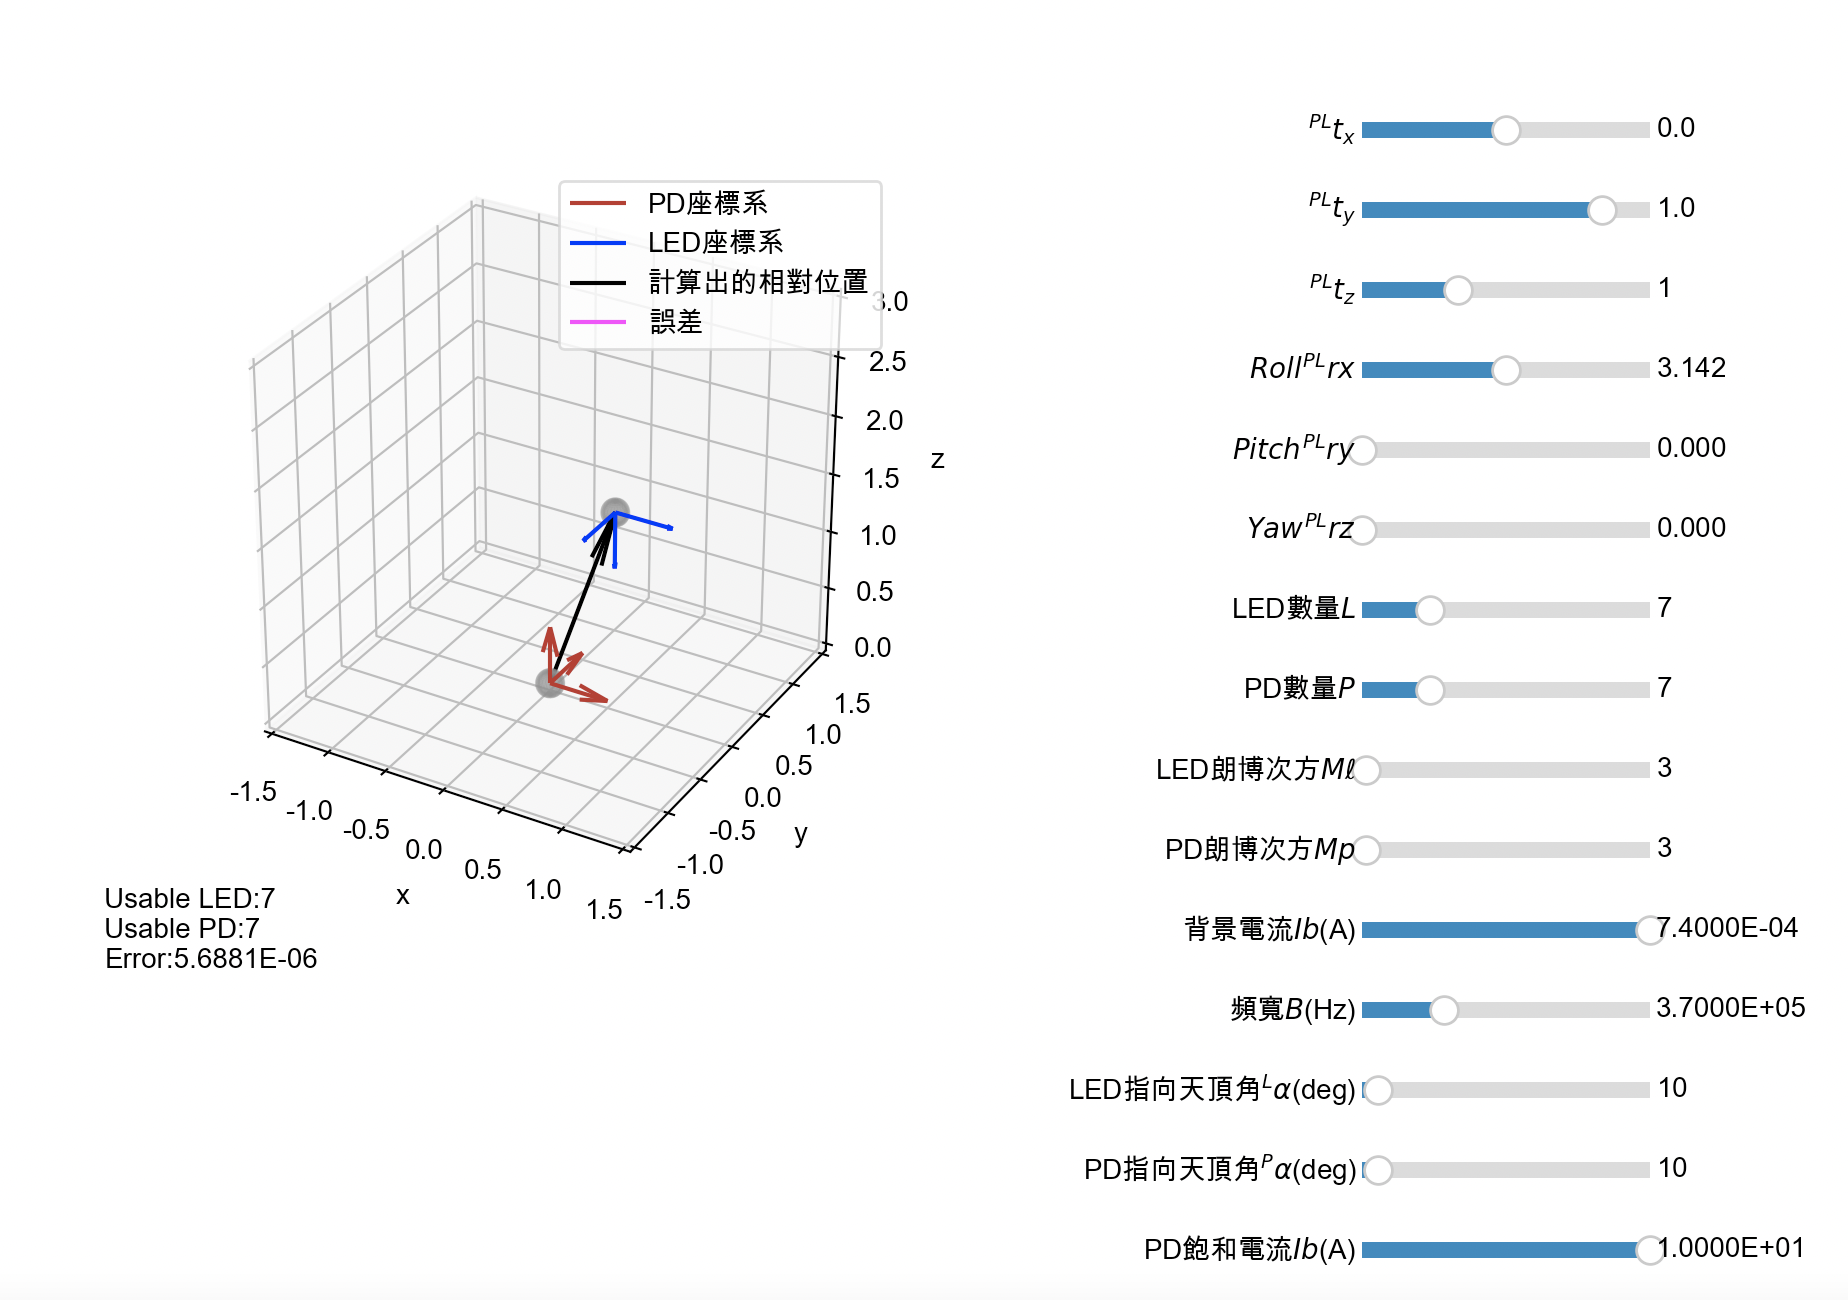
\includegraphics[width=15cm]{ch4pic/result_interactive.png}
    \caption{定位模擬結果互動介面}
    \label{pic:result_interactive}
\end{figure}



\begin{table}[htpb]
    \begin{center}
      \caption{於不同系統設置位置的定位結果}
      \label{tab:pos_error_result}
      \begin{tabular}{c||c|c|c|c|c|c||c} % <-- Alignments: 1st column left, 2nd middle and 3rd right, with vertical lines in between
         系統& $^{PL}t_x$ & $^{PL}t_y$&$^{PL}t_z$&$ ^{PL}rx$ & $^{PL}ry$&$^{PL}rz$&誤差\\
         設置& (m) & (m)&(m)&(rad) & (rad)&(rad)&(m)\\
        \hline
        (a)& 1.5 & 1&1&$\pi$ & 0&0&$2.079\times10^{-3}$\\
        (b)& 1.5 & 1&1&$\pi$ & 2.313&0&$3.723\times10^{-1}$\\
        (c)& 1.5 & 1&1&$\pi$ & 2.533&0&(無法求解)\\
        (d)& 1.5 & 1.5&3&$\pi$ & 0&0&$2.906\times10^{-1}$\\
      \end{tabular}
    \end{center}
  \end{table}

  \begin{figure}[htpb]
    \centering
    \begin{minipage}{.5\textwidth}
        \centering
        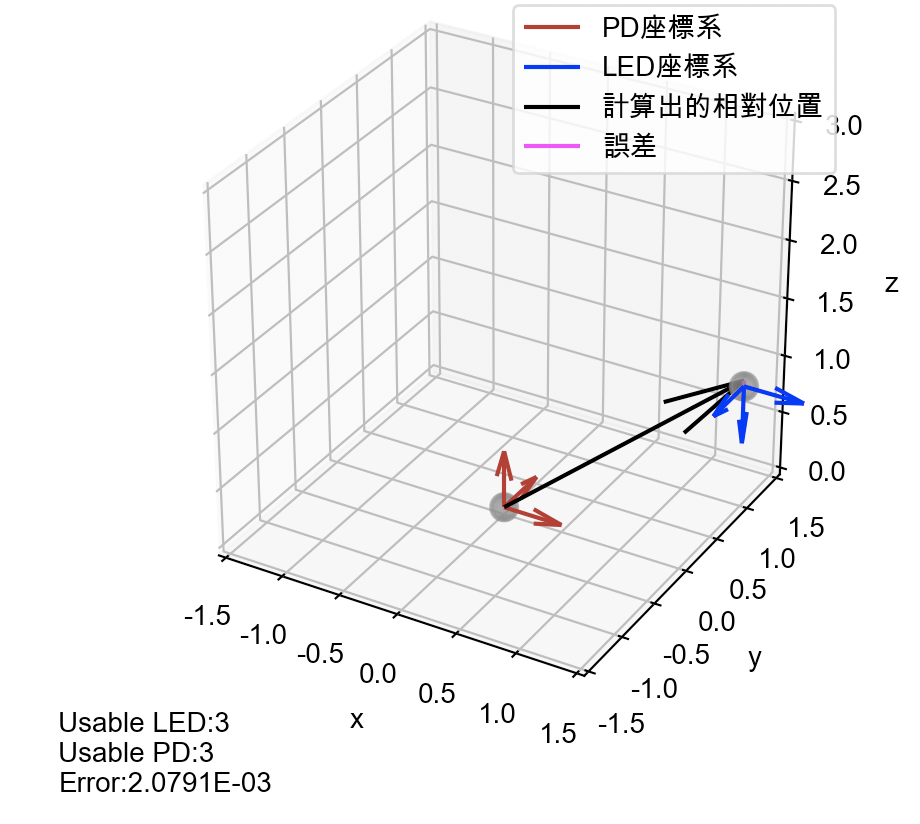
\includegraphics[width=7cm]{ch4pic/A.png}
        % \captionsetup{labelformat=empty}
        \caption{系統設置(a)的定位結果}
        \label{pic:A}
    \end{minipage}%
    \begin{minipage}{0.5\textwidth}
        \centering
        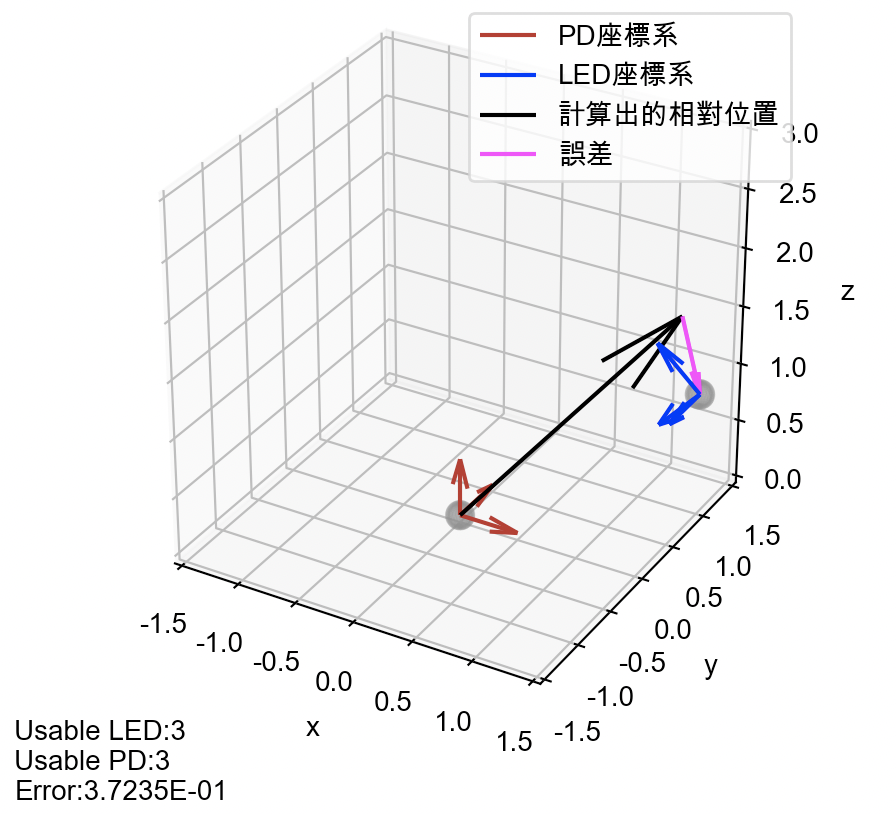
\includegraphics[width=7cm]{ch4pic/B.png}
        % \captionsetup{labelformat=empty}
        \caption{系統設置(b)的定位結果}
        \label{pic:B}
    \end{minipage}

\end{figure}

\begin{figure}[htpb]
    \centering
    \begin{minipage}{.5\textwidth}
        \centering
        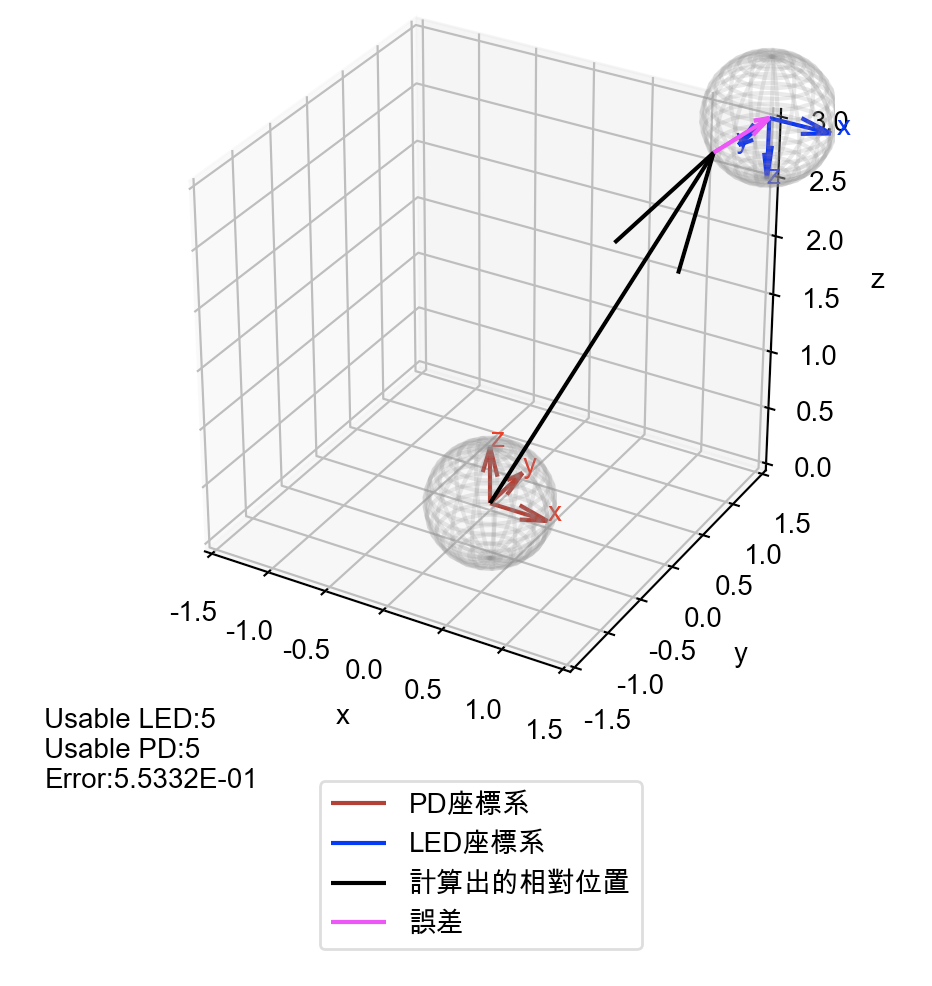
\includegraphics[width=7cm]{ch4pic/C.png}
        % \captionsetup{labelformat=empty}
        \caption{系統設置(c)的定位結果}
        \label{pic:C}
    \end{minipage}%
    \begin{minipage}{0.5\textwidth}
        \centering
        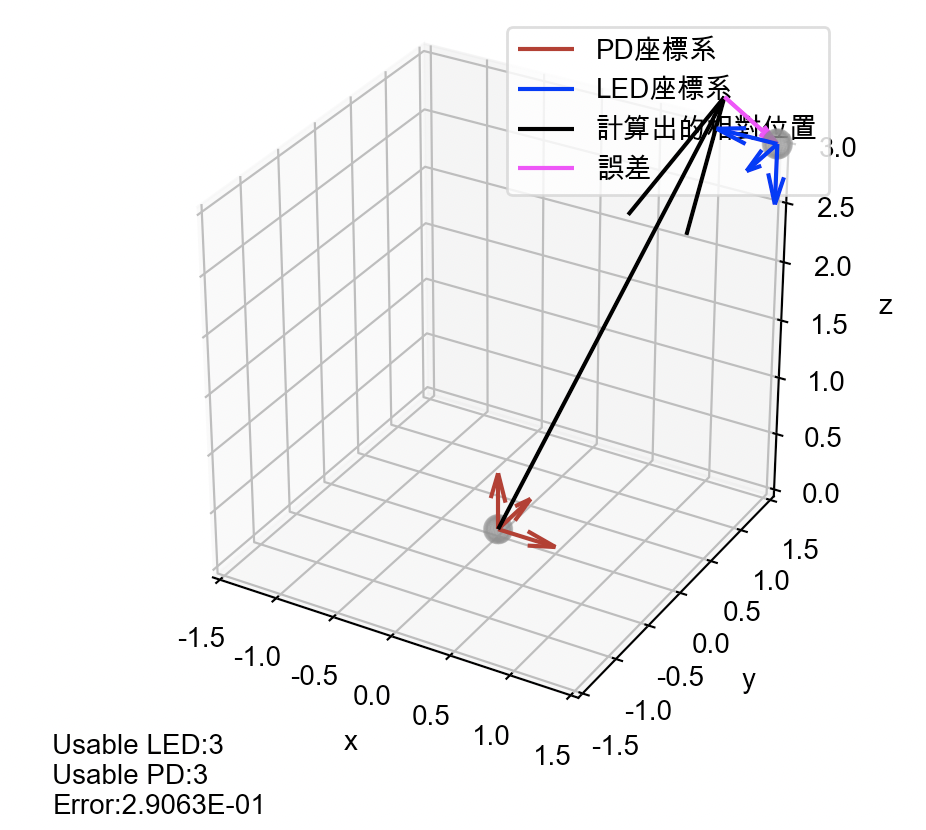
\includegraphics[width=7cm]{ch4pic/D.png}
        % \captionsetup{labelformat=empty}
        \caption{系統設置(d)的定位結果}
        \label{pic:D}
    \end{minipage}

\end{figure}


我們觀察改變Step2.系統設置的結果,系統設置的參數與誤差於表\ref{tab:pos_error_result}中呈現,系統架構則於圖\ref{pic:A}至圖\ref{pic:D}呈現,其中PD次系統以紅色座標軸表示,LED次系統則以藍色座標軸表示,透過\ref{chp:simulation}章中模擬方式所得到的相對位置以黑色向量表示,誤差向量則以粉色向量表示。

我們可以觀察到在同樣的次系統規格下,定位系統於不同系統設置的位置下,系統成效也不盡相同,如在系統設置為(c)時,由於沒有任何PD同時獲得三個以上的LED訊號,因此無法完成定位(參考\ref{chp:orient_conclu}章);而在系統設置為(a)時,則可以達到相對誤差小的定位。

除了系統設置的影響以外,不同的次系統規格與誤差模擬參數也都會對系統成效有不同程度的影響,為了更有效率的分析不同次系統規格的系統成效,以及了解不同參數對系統的影響,我們進一步於後續\ref{chp:system_evaluate}章中建立評估系統效能的流程,以便有系統性的討論不同次系統規格、系統設置、誤差模擬參數對系統成效的影響。

% \subsection{小結}

% 我們利用\ref{chp:simulation}章中的方法,帶入\ref{chp:simulate_para}章中的硬體參數,於\ref{chp:simulate_result_sub}章中呈現不同系統設計下的定位結果$\hat{^{PL}\boldsymbol{T}}$,並計算出定位誤差$\hat{e}$。得到誤差後,我們即可透過改變兩座標系的相對位置,來觀察該系統設計在不同位置上的定位表現,因此我們在\ref{chp:system_evaluate}章中進行系統評估。





\newpage

\section{定位系統效能評估}
\label{chp:system_evaluate}

上一章節中,我們能夠完整的以數值模擬方式,針對不同的次系統規格設計於不同的系統設置位置,執行定位演算法以及計算出誤差;而本章節則是要建立一評估系統成效的流程,評估流程整理於圖\ref{pic:evaluate_flow}。為與前述定位流程呼應,評估流程中以StepA.到StepC.進行系統效能評估,首先需於StepA.中設定使用情境與ROI中的樣本點,將各樣本點以Step1.到Step4.的室內定位流程得到定位解$^{PL}\boldsymbol{T}$,此室內定位流程包裝為系統效能評估中的StepB.;而評估的最後一個步驟則是StepC.量化評估系統效能。


\begin{figure}[htpb]
    \centering
    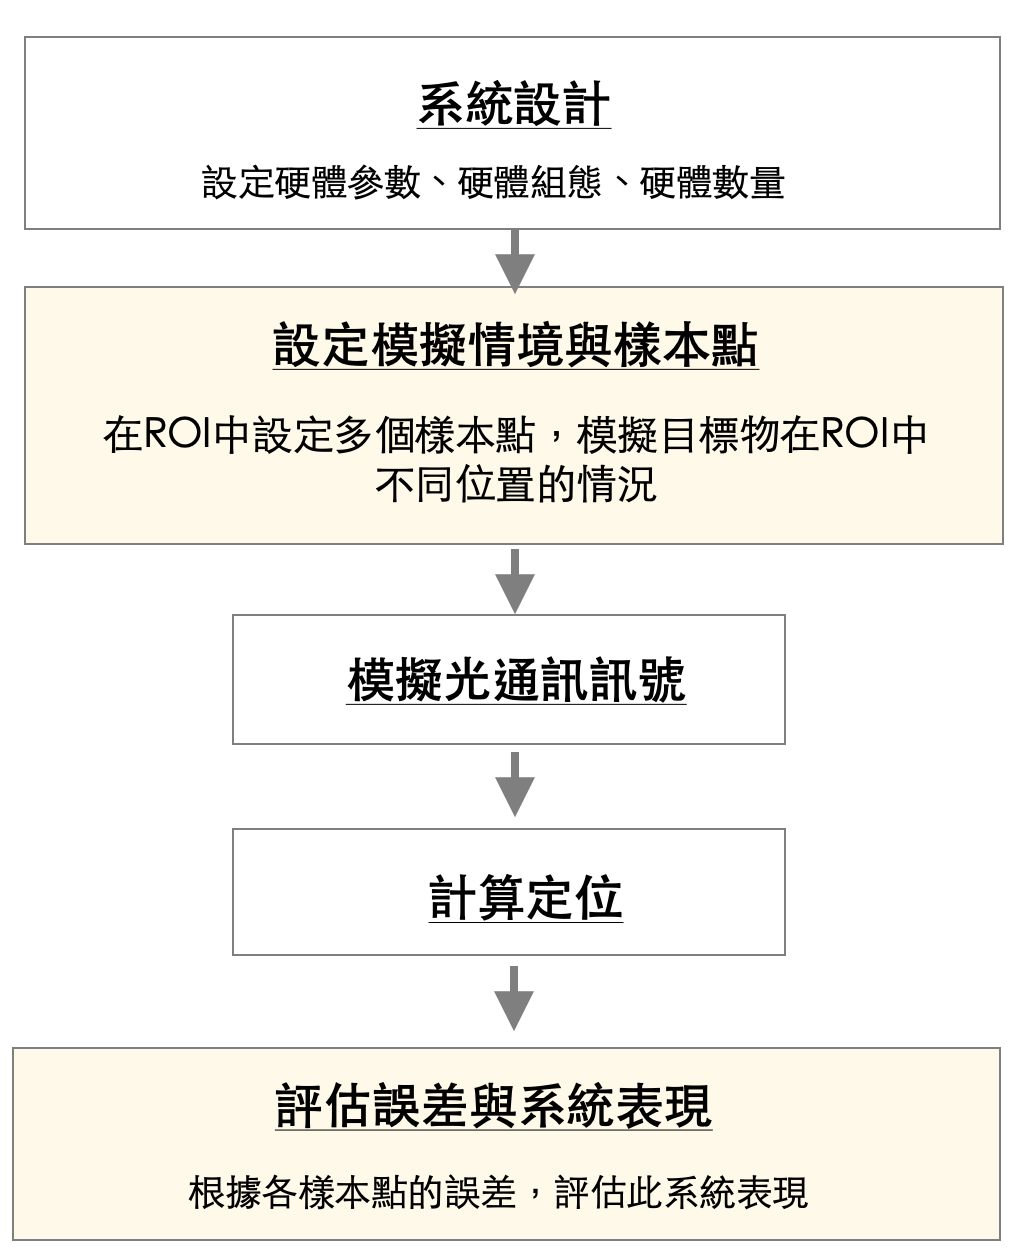
\includegraphics[width=10cm]{ch4pic/evaluate_flow.png}
    \caption{評估系統流程圖}
    \label{pic:evaluate_flow}
\end{figure}


以下依序由\ref{chp:scenario}章中介紹StepA.設定使用情境與ROI中樣本點,\ref{chp:system_evaluate}章中介紹StepC.量化評估系統效能的方法。

% 模擬流程中設定兩座標系相對關係的步驟一次計算一個位置的定位與誤差;而在評估系統設計時,我們須判斷環境中多個位置的誤差,以觀察該設計在不同位置的表現。因此評估時,我們需針對特定情境下感興趣範圍(Region of Interest,以下簡稱ROI)內的所有位置進行誤差計算,以建立多個樣本點的方式達到,詳述於\ref{chp:scenario}章中。而評估步驟的最後,則是對系統表現以\ref{chp:evaluate_method}章的方法進行量化與評估,系統設計的影響結果則於\ref{chp:design_result}章中分析。






\subsection{StepA.設定使用情境與ROI中樣本點}
\label{chp:scenario}




為了針對不同使用情境評估系統表現,我們須了解目標的使用情境並設定合適的ROI,而由於兩次系統之間的相對關係是透過齊次座標轉換矩陣定義(參考\ref{chp:simulate_position}章),描述LED座標系投影至PD座標系的轉換矩陣,因此ROI可以相對著PD座標系作定義,也就是將PD座標系視為參考點。透過目標使用情境設定ROI之後,我們需於其中建立多個樣本點,以多個樣本點來了解該次系統規格(Step1.)在ROI中不同系統設置(Step2.)時的表現,以進行系統評估。

在設定樣本點時以\ref{chp:simulate_position}章中表\ref{tab:para_relative}呈現的參數來定義系統設置,各樣本點的自由度包含平移與旋轉的各三個自由度。在這裡,我們選擇常見的室內定位情境作為模擬情境,也就是目標物LED座標系固定於天花板朝地面照射,而量測者的PD座標系於室內空間中。測試範圍則是設置為$3 \times 3 \times 3 m$的平移範圍。我們在此範圍內建立樣本點,平移自由度$^{PL}t_x$、$^{PL}t_y$、$^{PL}t_z$各自於範圍內平分為10段,總共有1000個平移樣本點。數值呈現於表\ref{tab:translate}中,於PD座標空間中的關係則呈現於圖\ref{pic:translate_sample}。

\begin{table}[htpb]
    \begin{center}
      \caption{平移樣本點}
      \label{tab:translate}
      \begin{tabular}{c|c|c|c} % <-- Alignments: 1st column left, 2nd middle and 3rd right, with vertical lines in between
         & \textbf{最小值} & \textbf{最大值}&\textbf{樣本數}\\
        \hline
        $^{PL}t_x$ & -1.5 & 1.5&10\\
        $^{PL}t_y$ & -1.5 & 1.5&10\\
        $^{PL}t_z$ & 0 & 3 &10\\
      \end{tabular}
    \end{center}
  \end{table}

\begin{figure}[htpb]
    \centering
    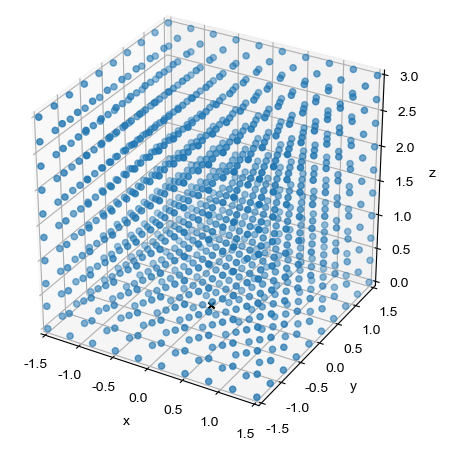
\includegraphics[width=6cm]{ch4pic/translate_sample.png}
    \caption{相對於PD座標系之平移樣本點}
    \label{pic:translate_sample}
\end{figure}

而由於本研究所使用的演算法並不需限制目標平面與量測平面平行,因此兩座標系之間的姿態也可以改變,除了平移的樣本點還需建立旋轉的樣本點,需定義Roll $^{PL}rx$、Pitch $^{PL}ry$、Yaw$^{PL}rz$三個參數。定義時,我們將Roll設定為$\pi$,使兩座標系呈現翻轉面對面的姿態。除了面對面姿態以外,其餘不平行旋轉樣本的設定參數呈現於表\ref{tab:rotate}中,共有61個旋轉樣本點。參考圖\ref{pic:rotate_sample},紅色箭頭代表的是PD座標系Z軸,藍色的各個箭頭則代表與其相對的的LED座標系Z軸,而Pitch與Yaw以極座標圖呈現於圖中。



\begin{table}[htpb]
    \begin{center}
      \caption{旋轉樣本點}
      \label{tab:rotate}
      \begin{tabular}{c|c|c|c} % <-- Alignments: 1st column left, 2nd middle and 3rd right, with vertical lines in between
        & \textbf{最小值} & \textbf{最大值}&\textbf{樣本數}\\
       \hline
       $^{PL}rx$ & $\pi$ & $\pi$&1\\
       $^{PL}ry$ & $\pi/18$ &$\pi/3$&6\\
       $^{PL}rz$ & $\pi/5$ & $2\pi$&10\\
     \end{tabular}
   \end{center}
 \end{table}

\begin{figure}[htpb]
    \centering
    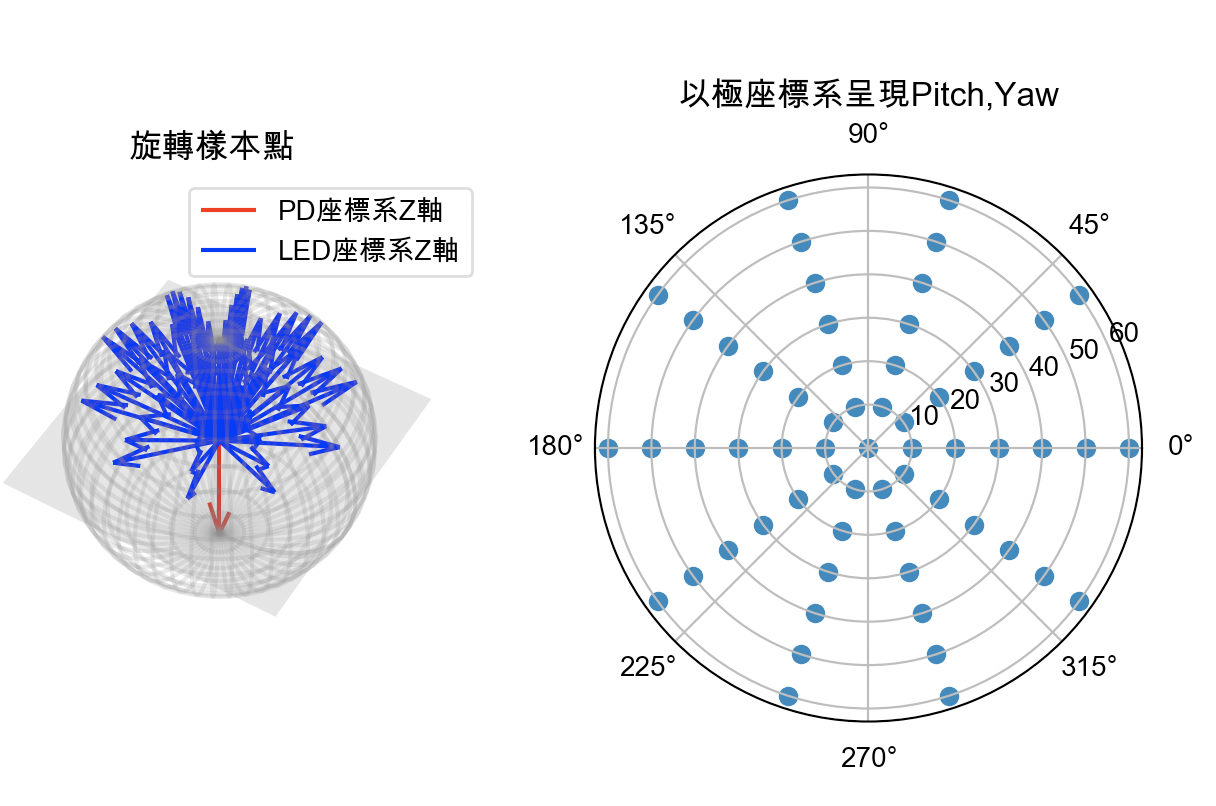
\includegraphics[width=12cm]{ch4pic/rotate_sample.png}
    \caption{相對於PD座標系之旋轉樣本點}
    \label{pic:rotate_sample}
\end{figure}


如表\ref{tab:translate}中所示,一共有$10\times 10\times 10$總共1000個平移樣本點,旋轉樣本點則有$1+1\times 6\times 10$共61個。這代表著每個平移樣本點上皆需做出61次旋轉,以旋轉樣本點來看也是,每個旋轉姿態都需在1000個平移樣本點上計算一次,兩者相乘代表總共61000個樣本點,我們以大寫$K$表示樣本點總數,而小寫$k$表示樣本點編號。






\subsection{量化系統表現}
\label{chp:evaluate_method}

於\ref{chp:scenario}章中建立了樣本點後,利用\ref{chp:simulation}章中的模擬方法對每個樣本點進行定位的計算,得到相對位置$\hat{_k^{PL}\boldsymbol{T}}$,並進行誤差$\hat{_k e}$的計算,參考示意圖\ref{pic:error_show},其中左下標k代表的是樣本點編號。

\begin{figure}[htpb]
    \centering
    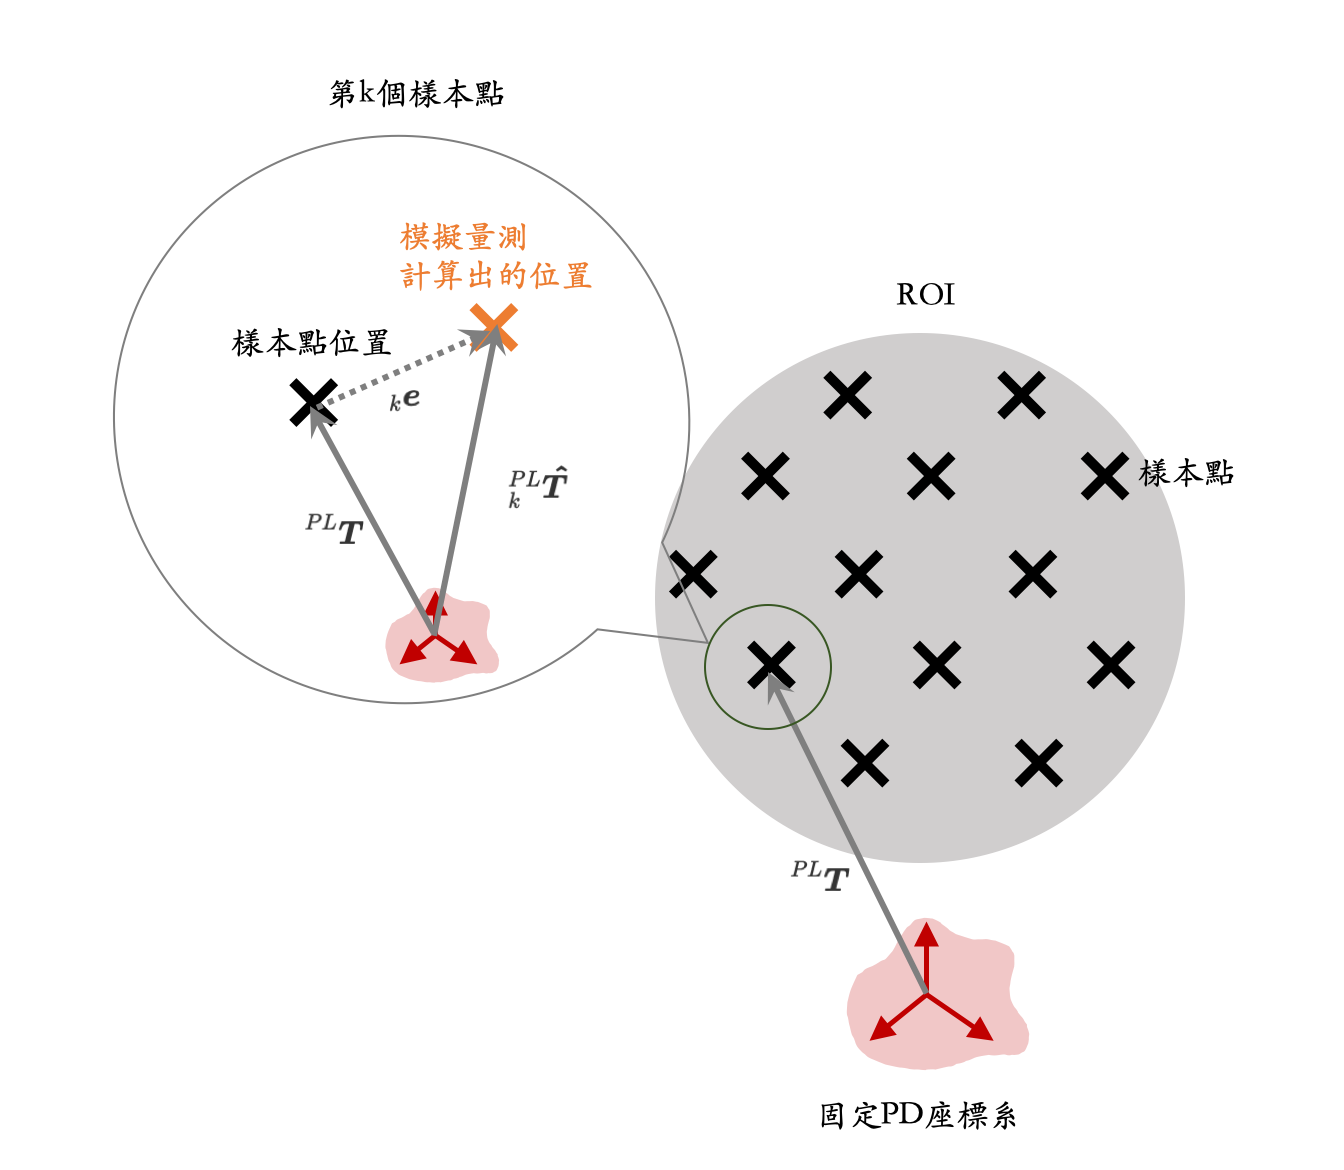
\includegraphics[width=9cm]{ch4pic/error.png}
    \caption{樣本點與誤差示意圖}
    \label{pic:error_show}
\end{figure}

\begin{gather}
    \label{eqn:sample_error}
    \hat{_k e} = ||^{PL}\boldsymbol{T}-\hat{^{PL}_k\boldsymbol{T}}||
\end{gather}



根據以上的情境設定,我們將61000個樣本點進行定位與誤差計算。其中,各樣本點可以如圖中的情況成功求解,獲得相對位置與誤差,各樣本點也有可能無法求解,因為該樣本點不滿足\ref{chp:orient_conclu}章中提到的演算法使用條件,也就是\textbf{沒有任何一個LED同時將訊號傳送給三個以上的PD,則無法解出方位;而若沒有任何一個PD同時接受到三個以上LED資訊,則無法計算距離}。即使我們今天系統設計有超過三個以上的LED與PD硬體數量,在\ref{chp:algorithm_filter}章中也會將訊號過大、過小的數值去除,導致所得訊號量不足求解的狀況。當有樣本點無法求解的情況時,我們無法計算定位誤差,所以無法僅用誤差來量化系統的表現。



因此,我們改以「在容許範圍$To$(Tolerance)內的樣本點數量」來量化描述系統成效,其中,可以將樣本點以平移樣本點與旋轉樣本點分別呈現,結果如圖\ref{pic:sample_out}。我們可以透過平移樣本點中容許範圍內的樣本點比例,觀察定位系統在不同平移相對位置上的表現,以圖\ref{pic:sample_out}來看,平移樣本點在距離PD座標系較近的位置擁有較好的系統成效;同樣我們也可以觀察不同旋轉樣本點上的系統成效,在圖\ref{pic:sample_out}的情況下,Pitch的角度越接近0時系統成效越好,也就是在目標物與觀察者平面平行時具有較好的系統成效。

\begin{figure}[htpb]
    \centering
    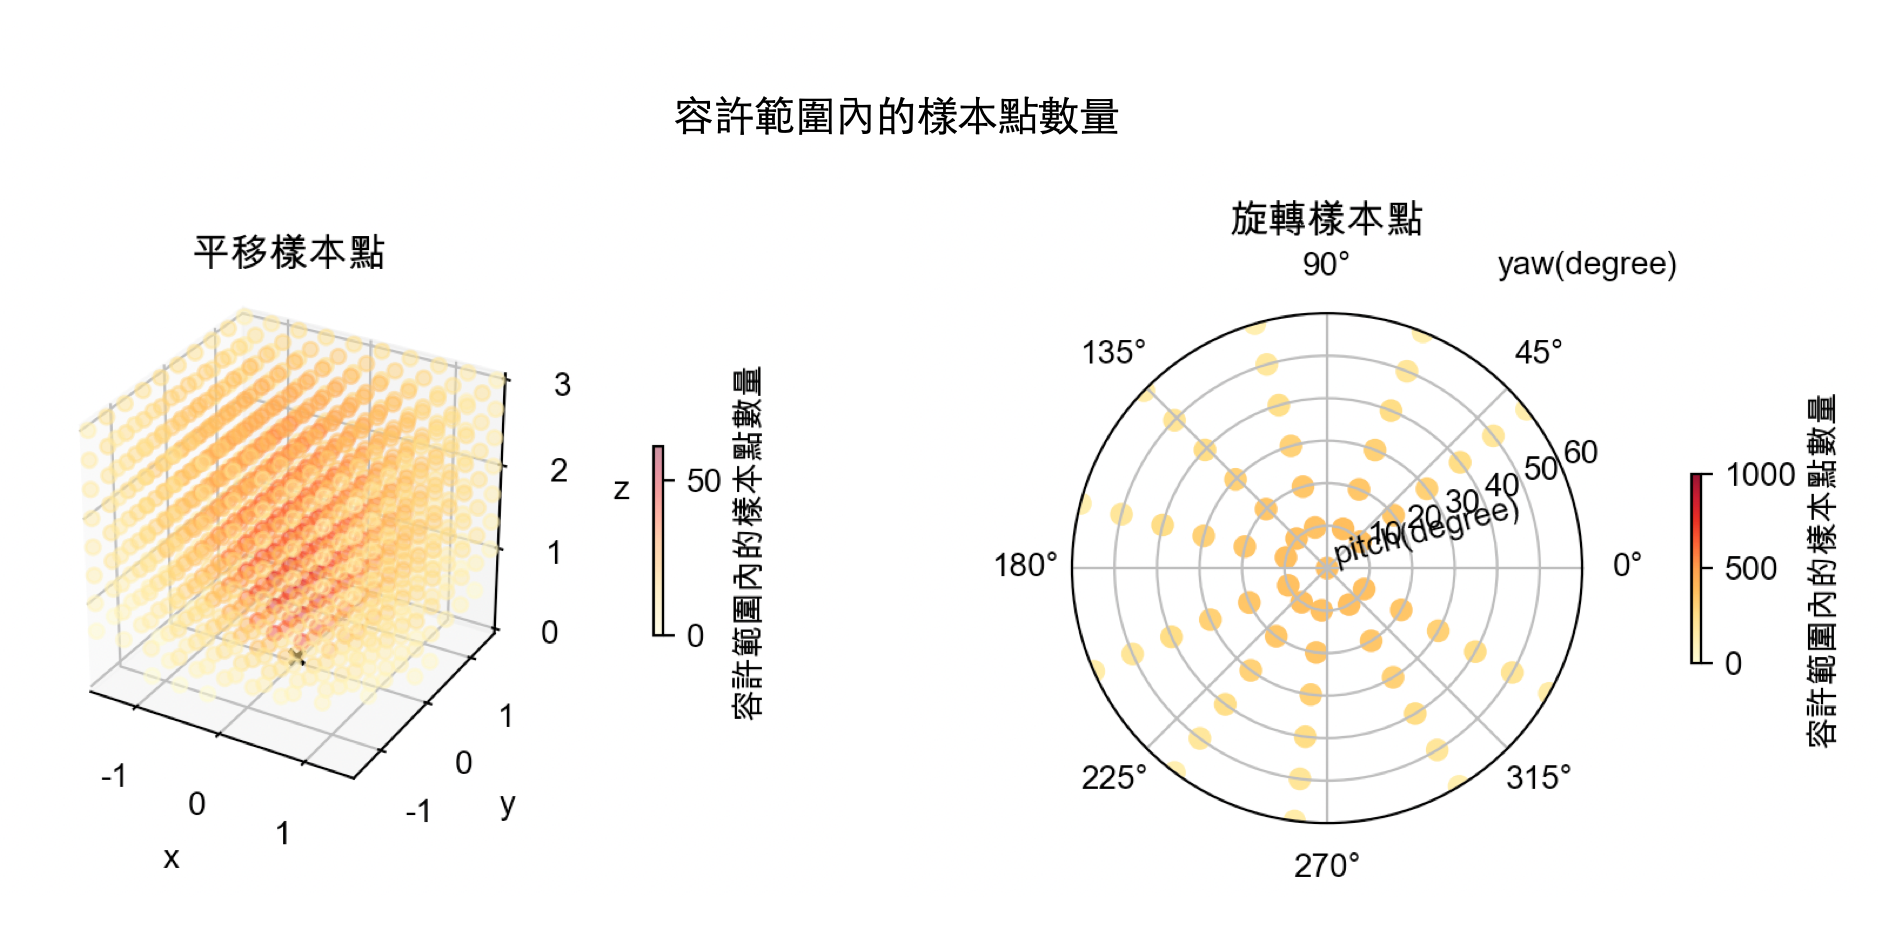
\includegraphics[width=14cm]{ch4pic/tolerance.png}
    \caption{容許範圍內的樣本點比例}
    \label{pic:sample_out}
\end{figure}

而由於樣本點數量多,僅透過容許範圍內的樣本點比例圖,仍無法非常清晰的看出系統於不同樣本位置的表現,因此圖\ref{pic:effective}則將圖\ref{pic:sample_out}中,於容許範圍內的比例超過有效閥值$Ef$的樣本點標示出,在這邊我們設定$Ef=80\%$。由圖\ref{pic:effective},我們可以更清楚的觀察到系統於哪些樣本點位置有較好的定位成效。

\begin{figure}[htpb]
    \centering
    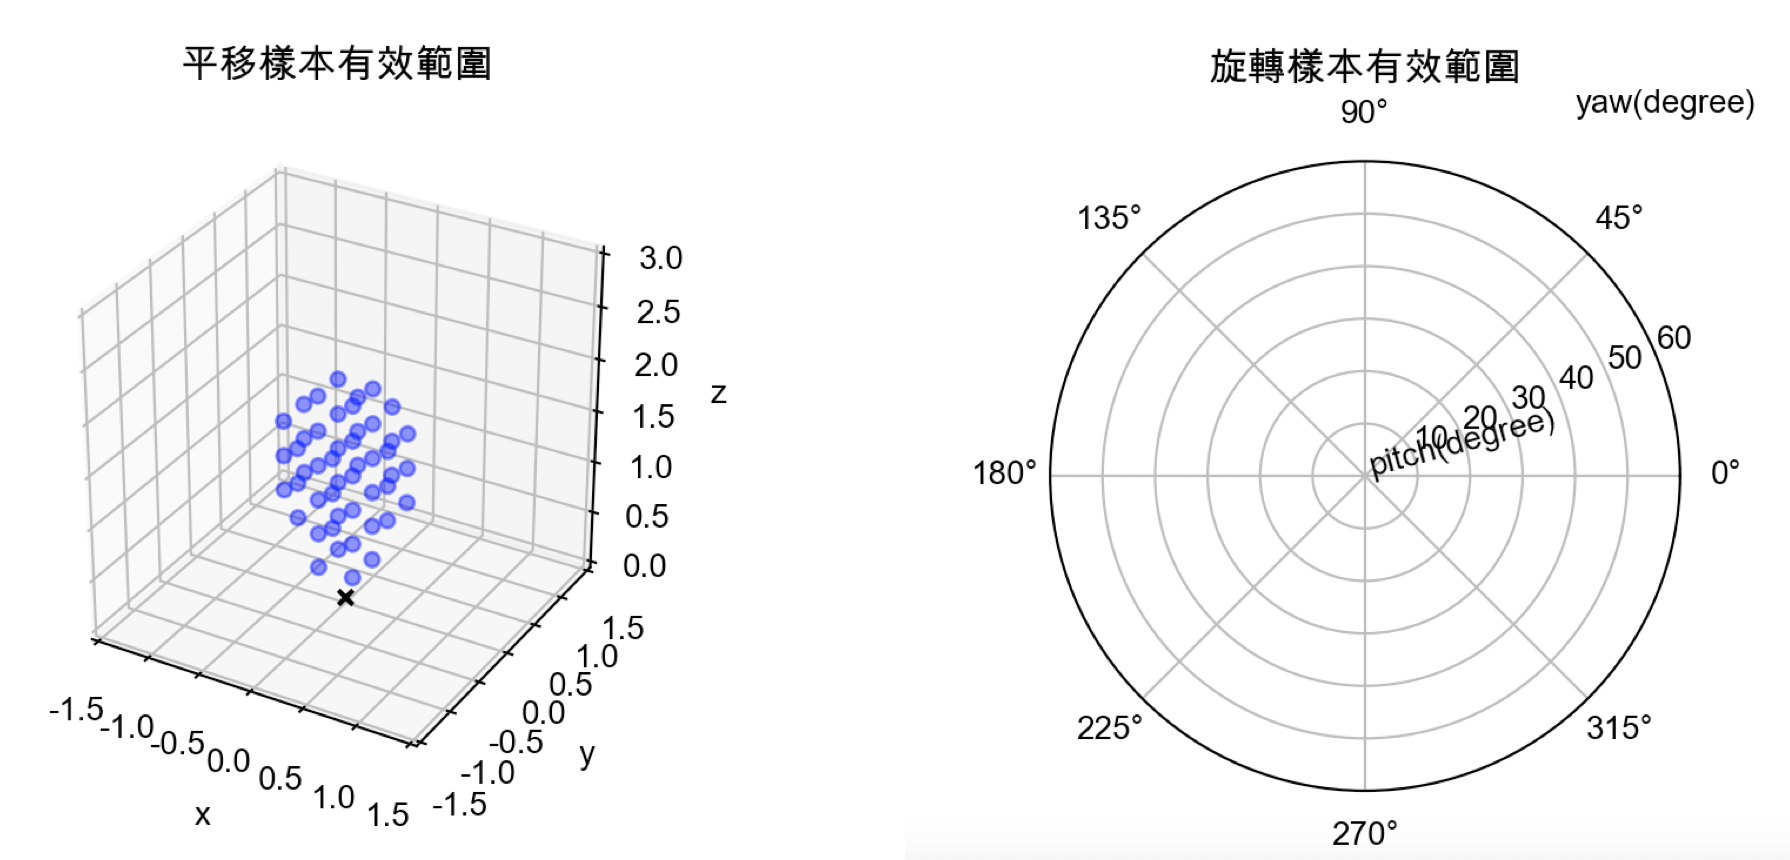
\includegraphics[width=14cm]{ch4pic/effective.png}
    \caption{樣本點中的有效範圍}
    \label{pic:effective}
\end{figure}



為了觀察不同現象的影響,我們一樣建立一個互動模擬介面如圖\ref{pic:analysis_interactive},可以透過改變不同的參數與變數,針對\ref{chp:scenario}章中設定的ROI進行評估。

\begin{figure}[htpb]
    \centering
    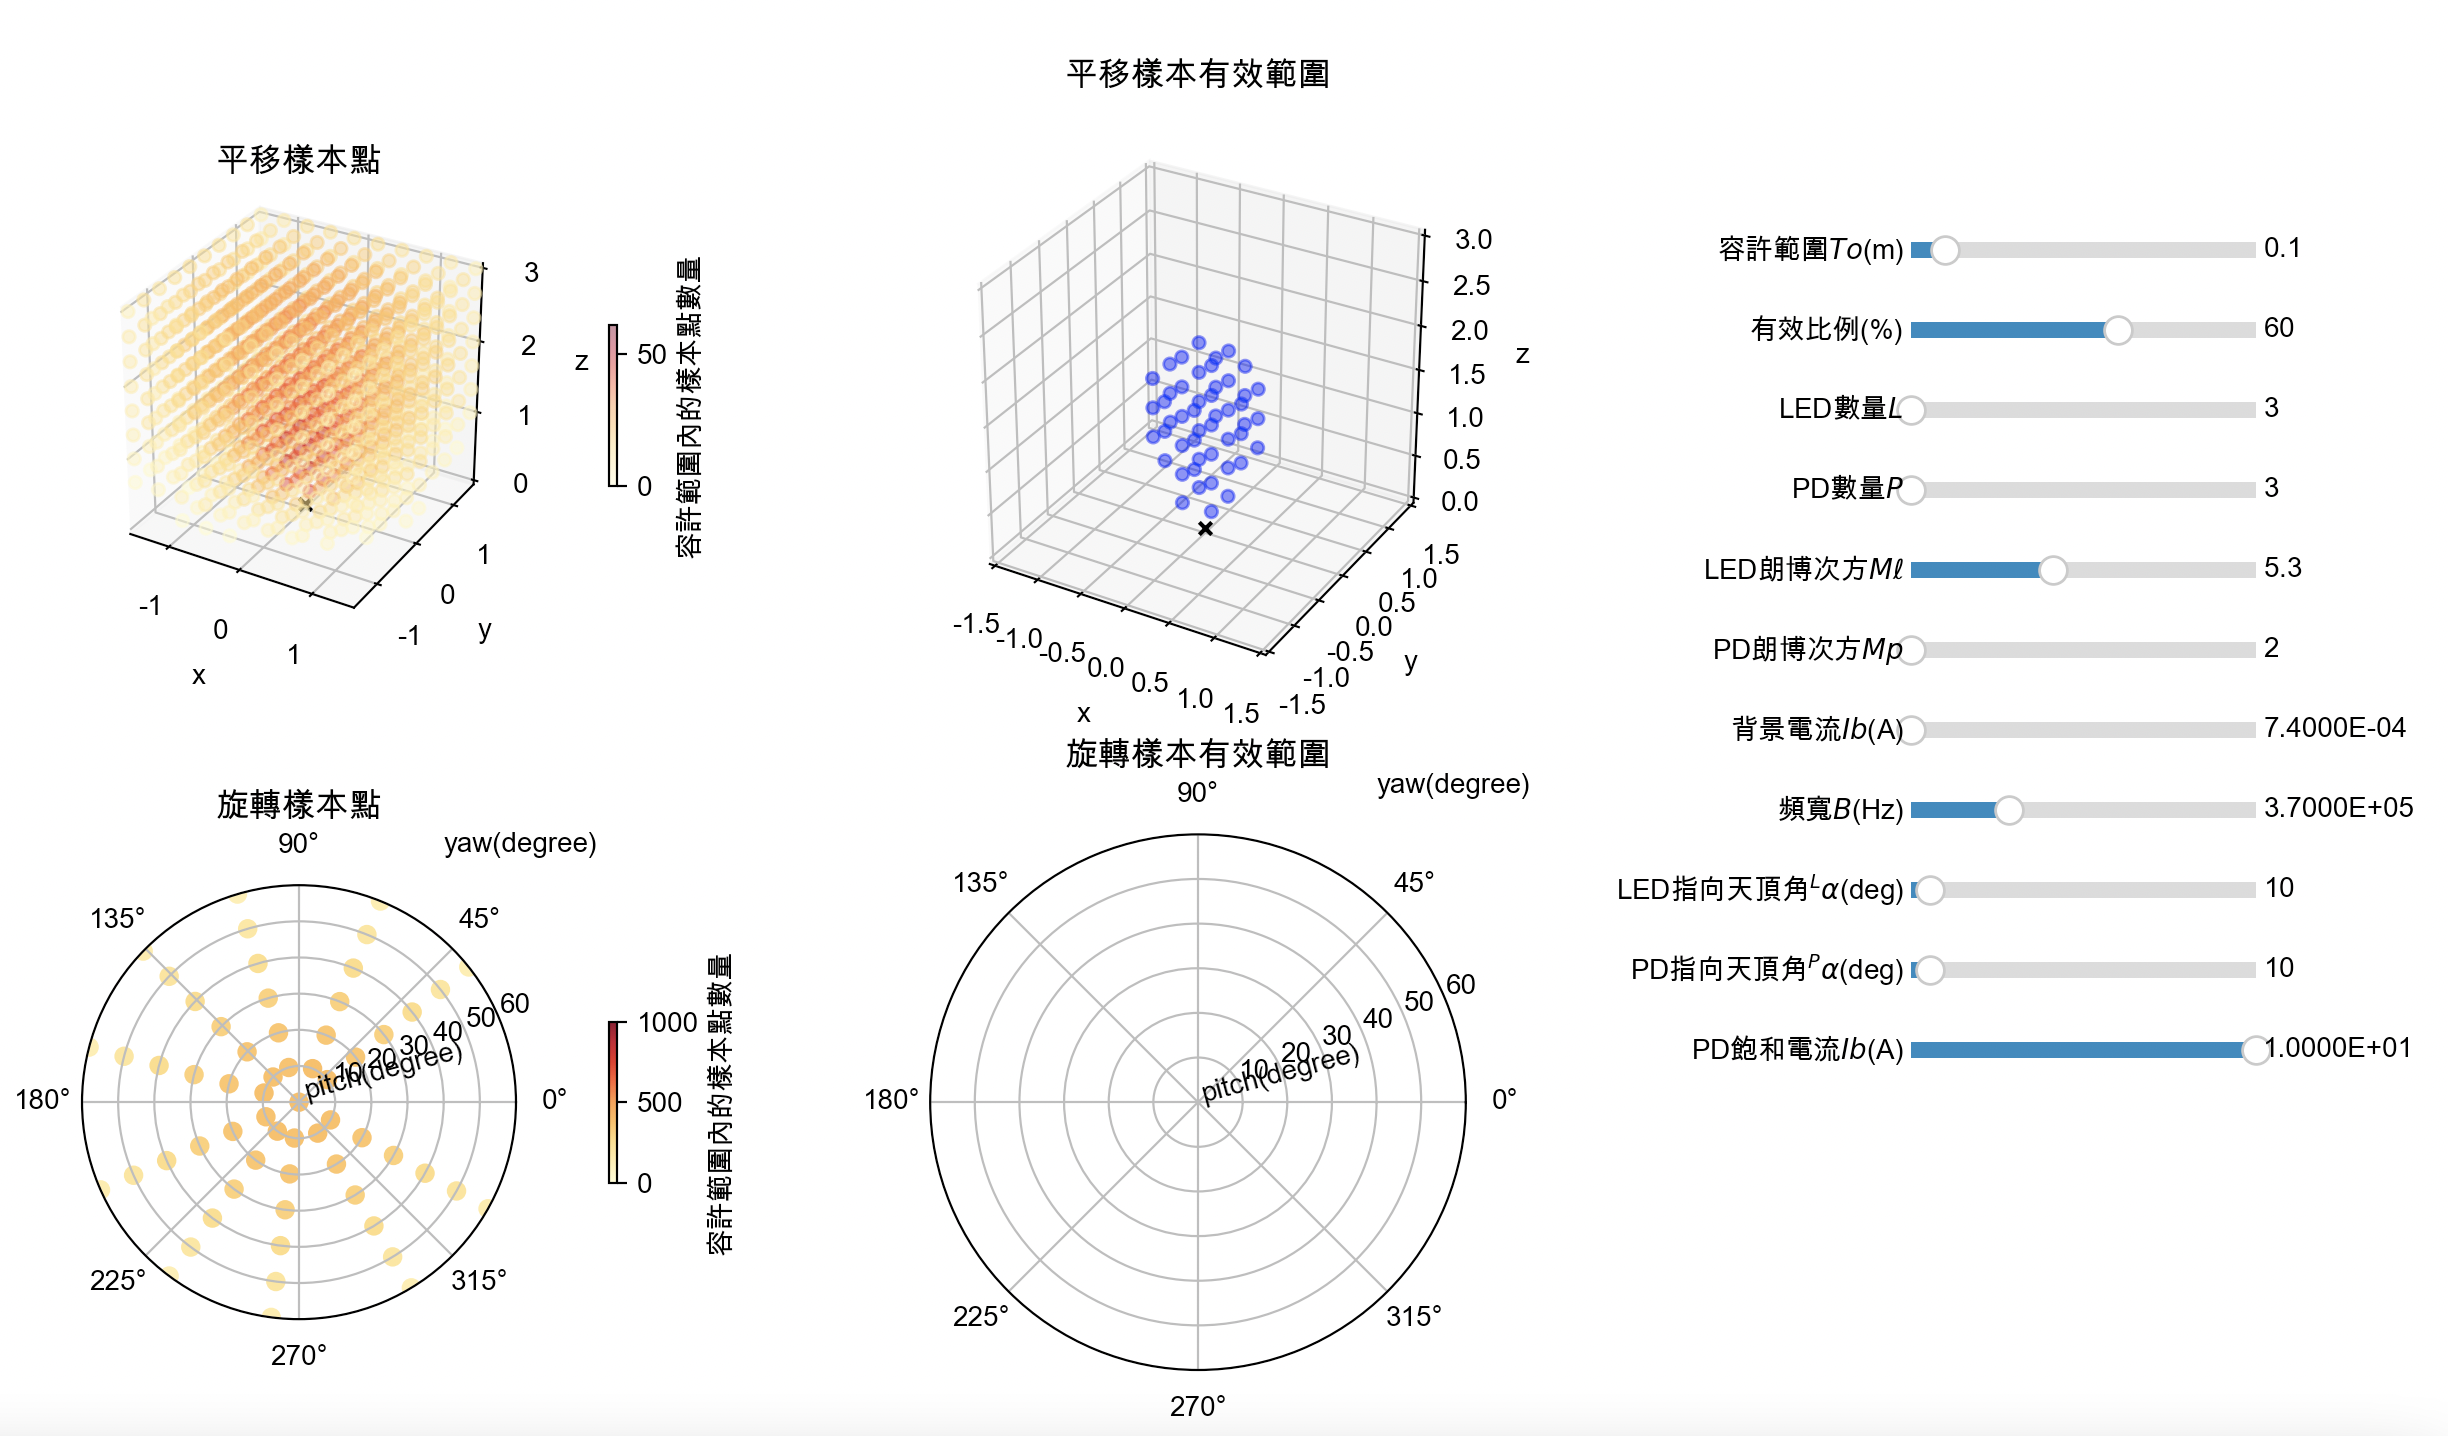
\includegraphics[width=15cm]{ch4pic/analysis_interactive.png}
    \caption{分析互動模擬介面}
    \label{pic:analysis_interactive}
\end{figure}

我們於後續章節透過調整不同參數,來觀察不同參數對系統成效的影響。

% 而由於第三章此演算法並沒有限制硬體數量、朗博次方與硬體指向,在設計上是有靈活度的,因此我們透過改變這幾項變數,來觀察系統的反應。其中,LED與PD指向的部分,我們將每個硬體皆具有的兩個由度限制剩下一個,假設方位角平均分配:$^P\beta_p = 2\pi/P$、$^L\beta_l = 2\pi/L$,仰角的部分則限制必須相同$^P\alpha_p =^P\alpha$、$^L\alpha_l = ^L\alpha$。在這樣的限制下,我們分別探討各項變數的影響。



\subsection{次系統規格對系統成效的影響}
\label{chp:design_result}

如\ref{chp:system_design}章中描述的,在Step1.決定次系統規格時,需決定硬體總數$L,P$、硬體規格參數、硬體指向。

在此段落,為了方便模擬,我們將LED硬體指向共$2L$個自由度,透過常見的指向限制(可參考\ref{chp:LEDPD_restrict}章)使,假設方位角平均分配:$^L\beta_l = 2\pi/L$,仰角的部分則限制各LED必須相同:$^L\alpha_l = ^L\alpha$,使$2L$個自由度降低為一個自由度:$^L\alpha$;而PD指向也用同樣的方法使$2P$個自由度僅剩下$^P\alpha$一個變數。

而硬體規格中的多項參數,並不是可以自由設計的參數,於\ref{chp:system_design}中我們參考硬體規格表中的參數進行模擬。然而,市售的LED與PD規格非常多種,我們難以將所有硬體規格輸入模擬系統進行評估,因此,我們挑選硬體參數中不能透過改變電路電壓電流進行調整的朗博次方參數作為代表硬體規格的變數,其代表著對出入射角敏感度與覆蓋範圍的取捨,可參考\ref{chp:lambertian}章。

因此,本段落針對Step1.次系統規格進行評估的變數包含:
\begin{enumerate}
    \item 定義LED硬體指向的天頂角$^L\alpha$
    \item 定義PD硬體指向的天頂角$^P\alpha$
    \item 代表LED硬體規格的LED朗博次方$M\ell$
    \item 代表PD硬體規格的PD朗博次方$Mp$
    \item LED硬體總數$L$
    \item PD硬體總數$P$

\end{enumerate}

以下於\ref{chp:orient_effect}章至\ref{chp:amount_effect}章中進行討論。











\subsubsection{朗博次方對系統成效的影響}
\label{chp:m_effect}

在討論朗博次方對系統成效的影響時,我們將其餘系統設計變數固定:假設$^P\alpha_p =^L\alpha_l = \pi/18$、$L=P=5$,透過改變朗博次方,將不同LED與PD朗博次方的次系統規格下,計算容許範圍內樣本點的數量,以圖\ref{pic:}呈現平移樣本點與圖呈現旋轉樣本點受朗博次方的影響。

\begin{figure}[htpb]
    \centering
    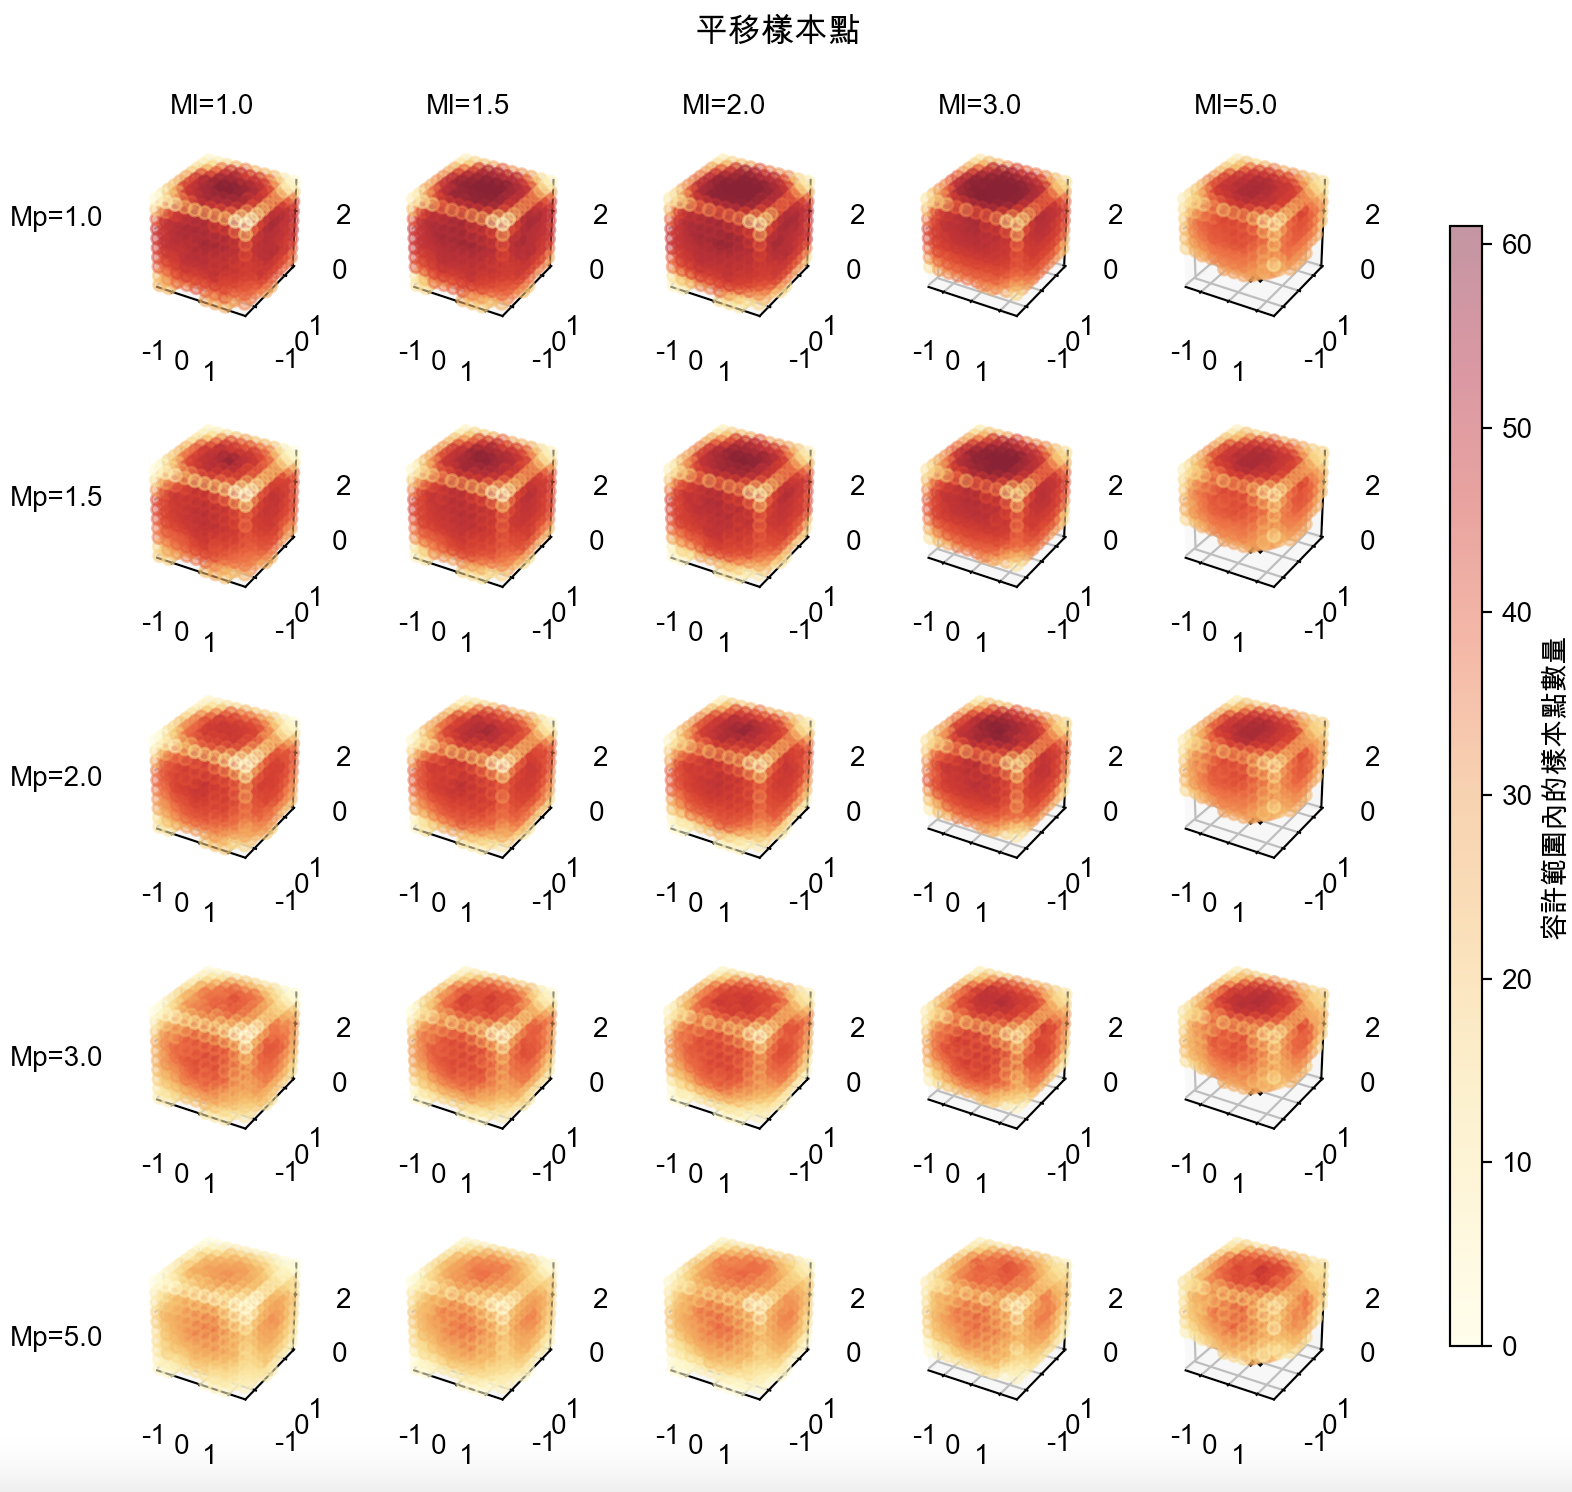
\includegraphics[width=14cm]{ch4pic/lambertian_translate.png}
    \caption{改變朗博次方對平移樣本點的影響}
    \label{pic:m_translate}
\end{figure}
\begin{figure}[htpb]
    \centering
    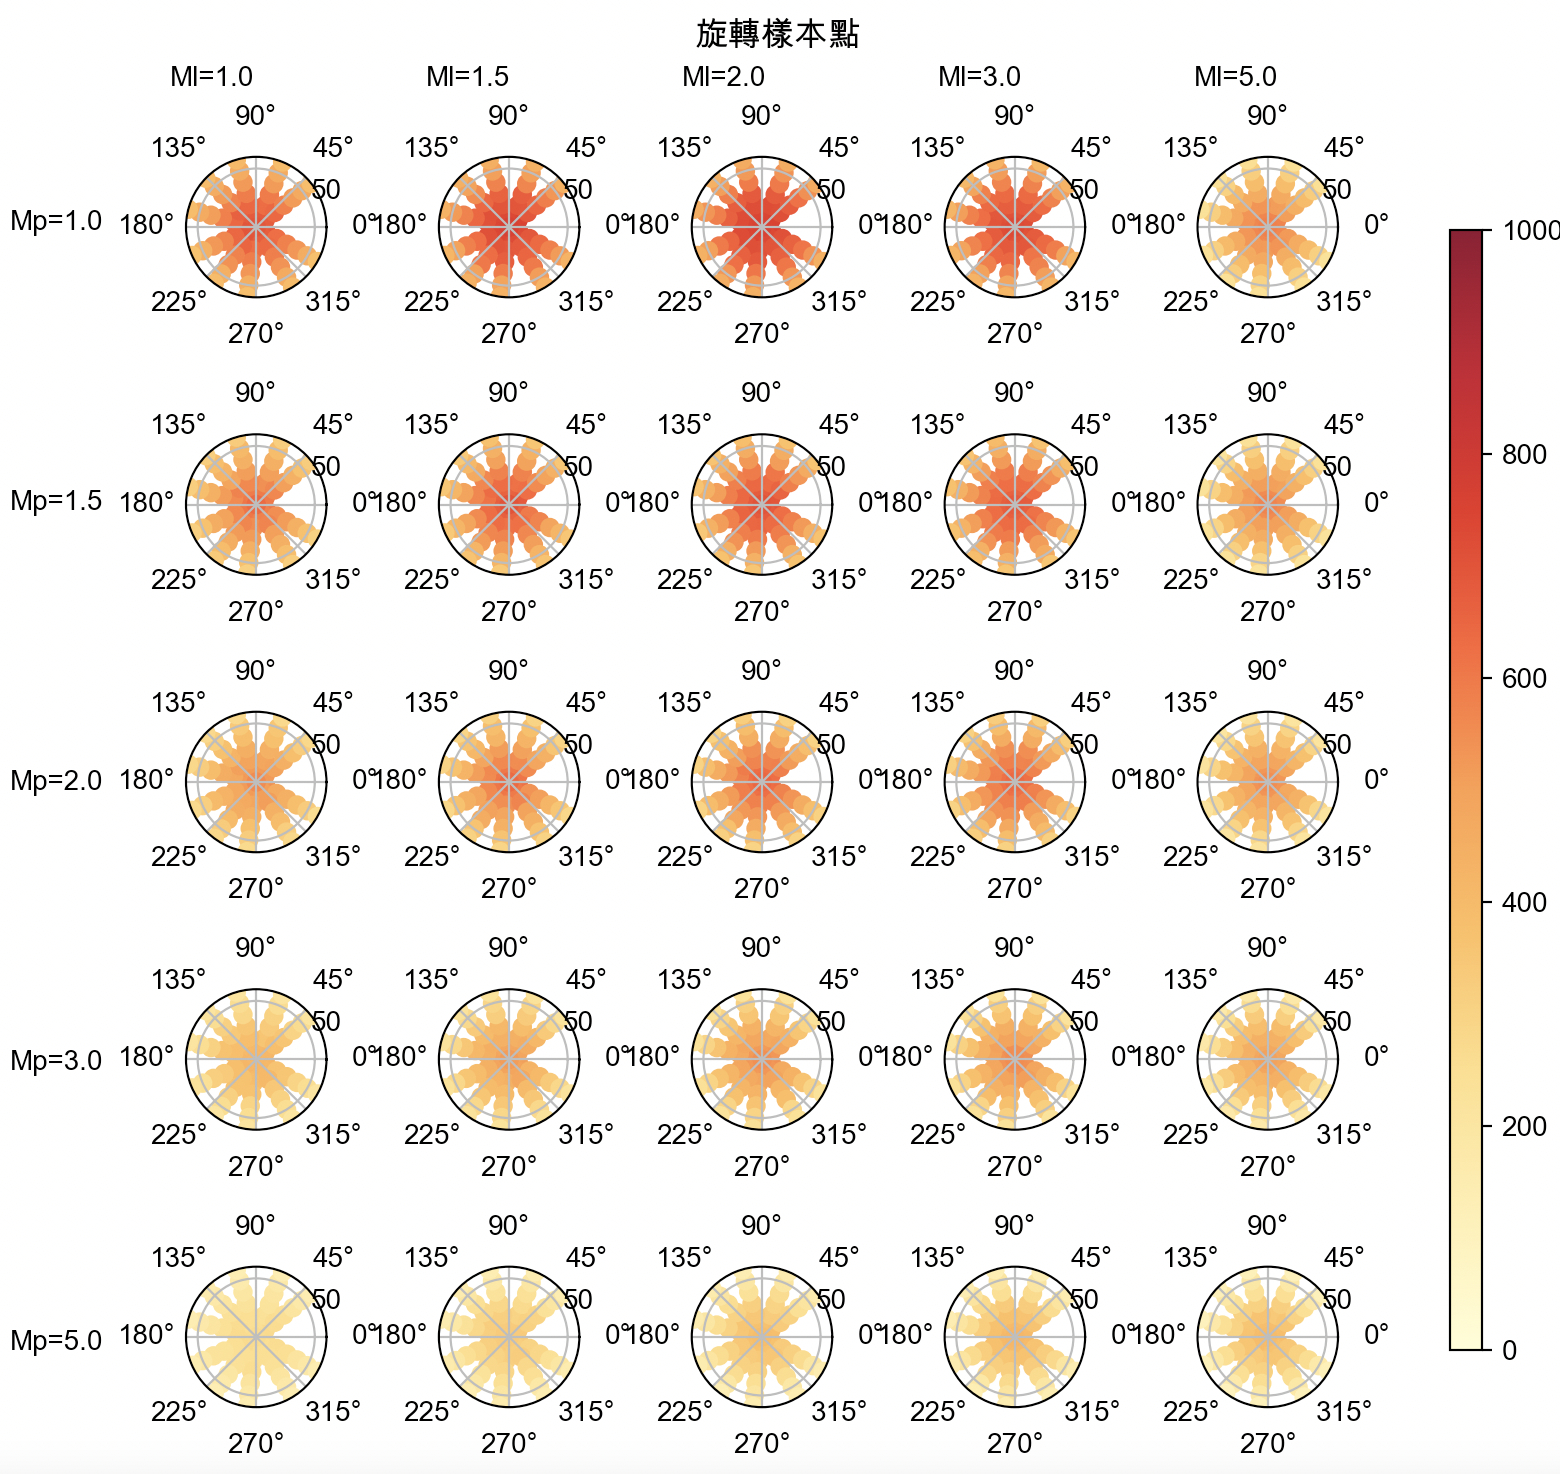
\includegraphics[width=14cm]{ch4pic/lambertian_rotate.png}
    \caption{改變朗博次方對旋轉樣本點的影響}
    \label{pic:m_rotate}
\end{figure}

在,以及硬體數量的情況下,我們將平移與旋轉樣本點總共六萬個點中,在容許範圍內的比例,呈現於圖\ref{pic:m_effect},我們可以觀察到在此情境中,較小的朗博次方使系統表現較佳。
% 我們改變朗博次方,並將樣本中於容許範圍內的比例,
% 呈現於圖\ref{pic:m_translate}與圖\ref{pic:m_rotate}中。隨著朗博次方的提升,硬體所照射的範圍越來越小,因此容許範圍內比例高的的區域便越顯集中。





\begin{figure}[htpb]
    \centering
    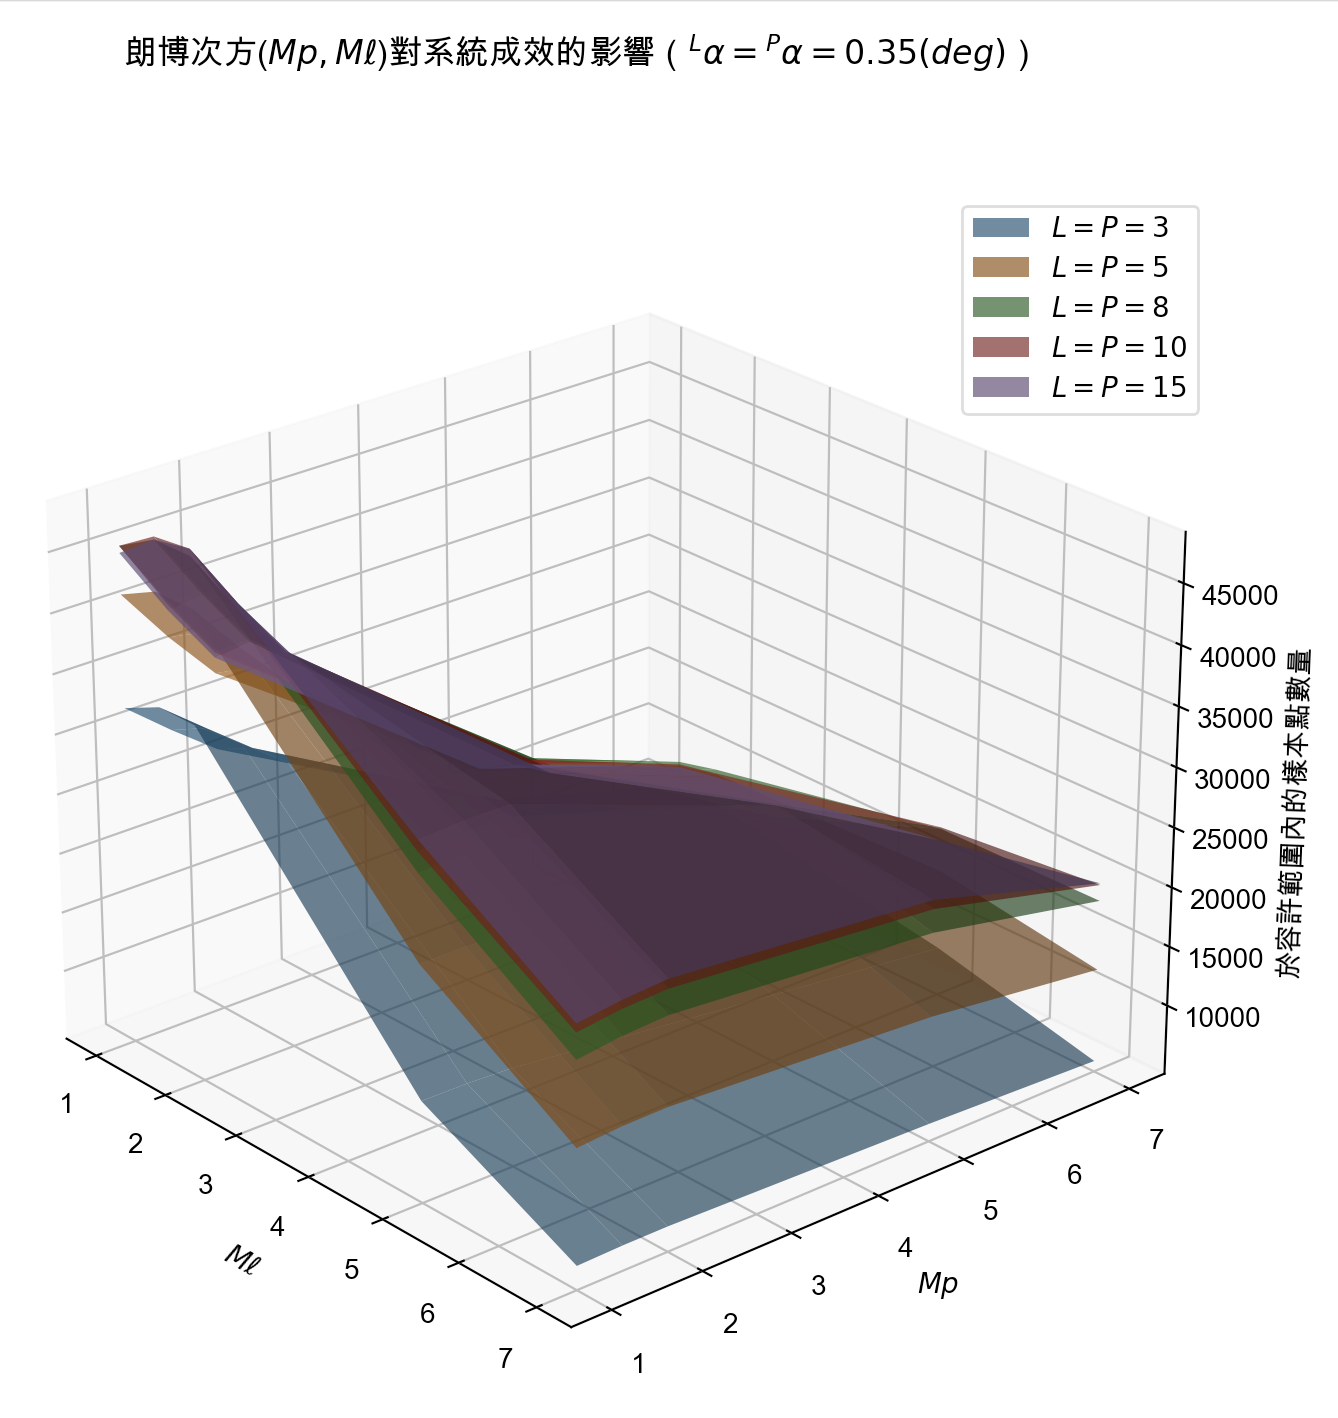
\includegraphics[width=9cm]{ch4pic/m_effect.png}
    \caption{改變朗博次方對系統的影響}
    \label{pic:m_effect}
\end{figure}

\subsubsection{硬體指向對系統效能的影響}
\label{chp:orient_effect}

評估硬體指向對系統效能影響時,我們將硬體天頂角$^L\alpha$與$^P\alpha$作為變數,其餘的變數:朗博次方固定為$Mp=M\ell=1$、硬體數量設定為$L=P=5$


將不同硬體天頂角的次系統規格,計算出的於容許範圍內的樣本點總數,呈現於圖\ref{pic:alpha_effect}

其餘朗博次方固定為$Mp=M\ell=1$,而硬體數量$L=P$則依序由3、5、8、10、15遞增,我們改變硬體指向$^P\alpha,^L\alpha$,我們將平移與旋轉樣本點總共六萬個點中,在容許範圍內的比例,呈現於圖\ref{pic:alpha_effect},我們可以觀察到在此情境中,較小的硬體擺設天頂角,使系統表現較佳。
% 並將樣本中於容許範圍內的比例,呈現於圖\ref{pic:alpha_translate}與圖\ref{pic:alpha_rotate}中。隨著硬體指向提升,多個硬體之間重疊的覆蓋範圍便越來越小,漸漸僅剩下於中心位置的樣本點:$x,y,=0$。

% \begin{figure}[htpb]
%     \centering
%     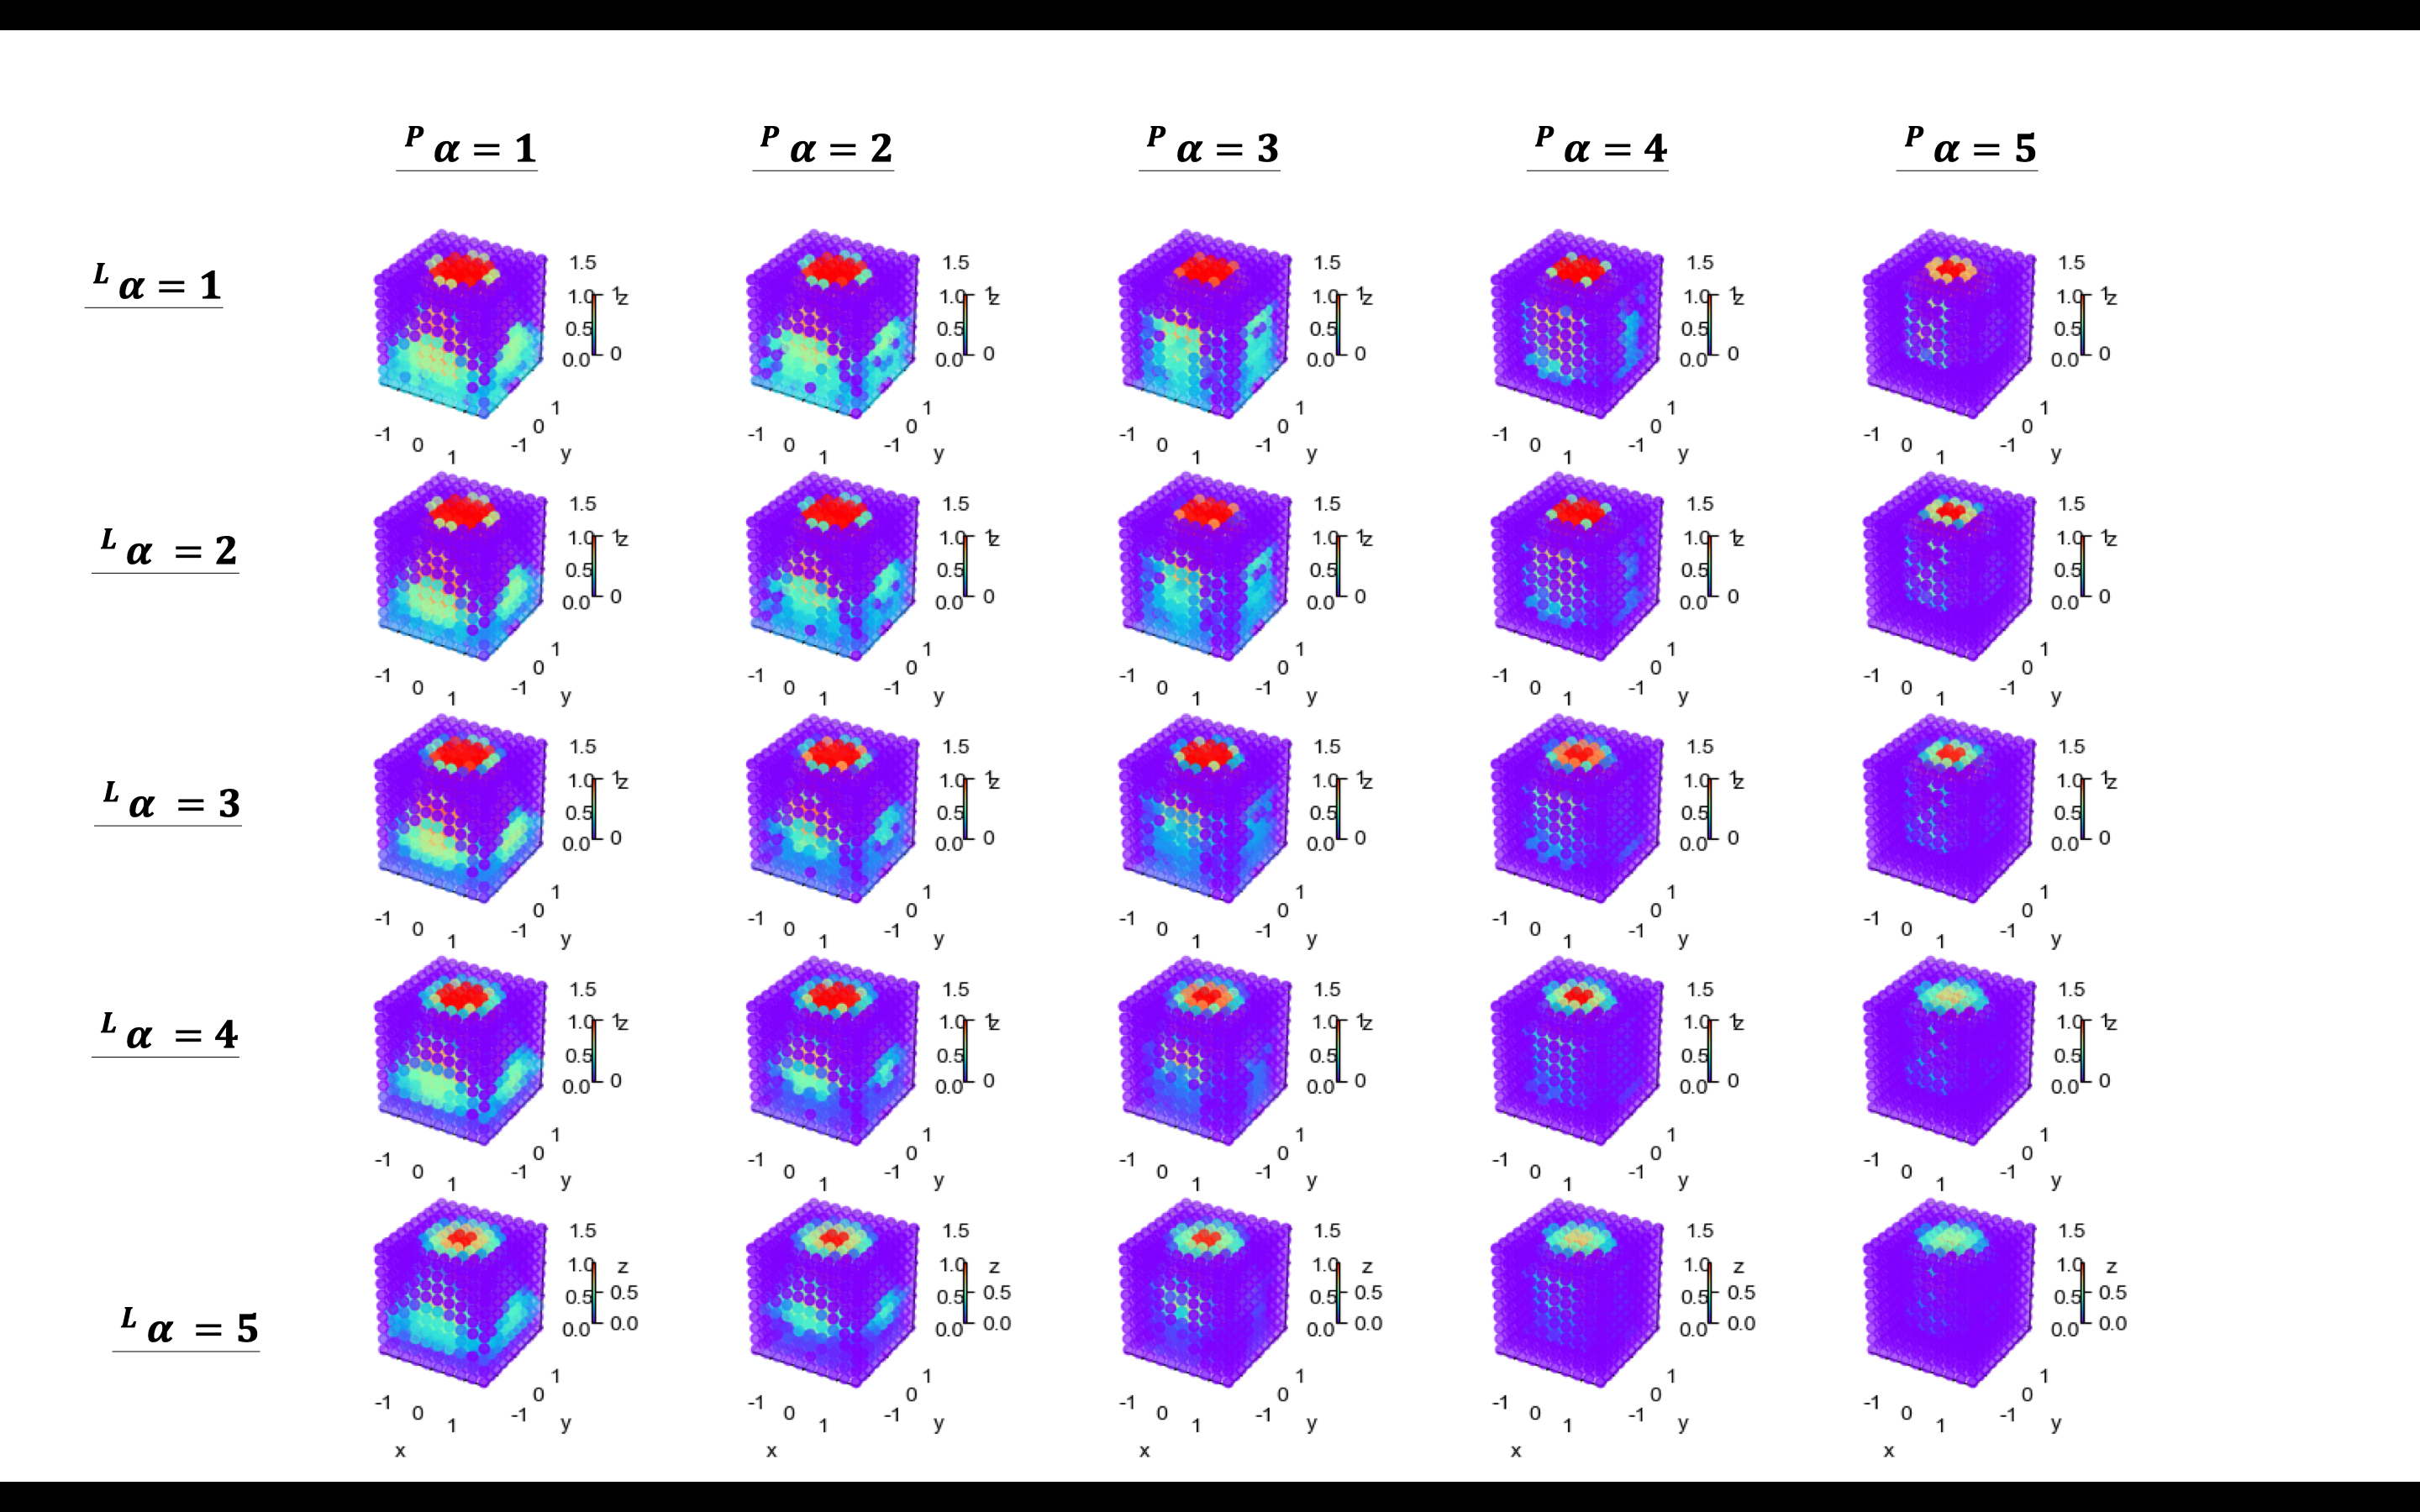
\includegraphics[width=14cm]{ch4pic/alpha_translate.png}
%     \caption{改變硬體指向對平移樣本點的影響}
%     \label{pic:alpha_translate}
% \end{figure}
% \begin{figure}[htpb]
%     \centering
%     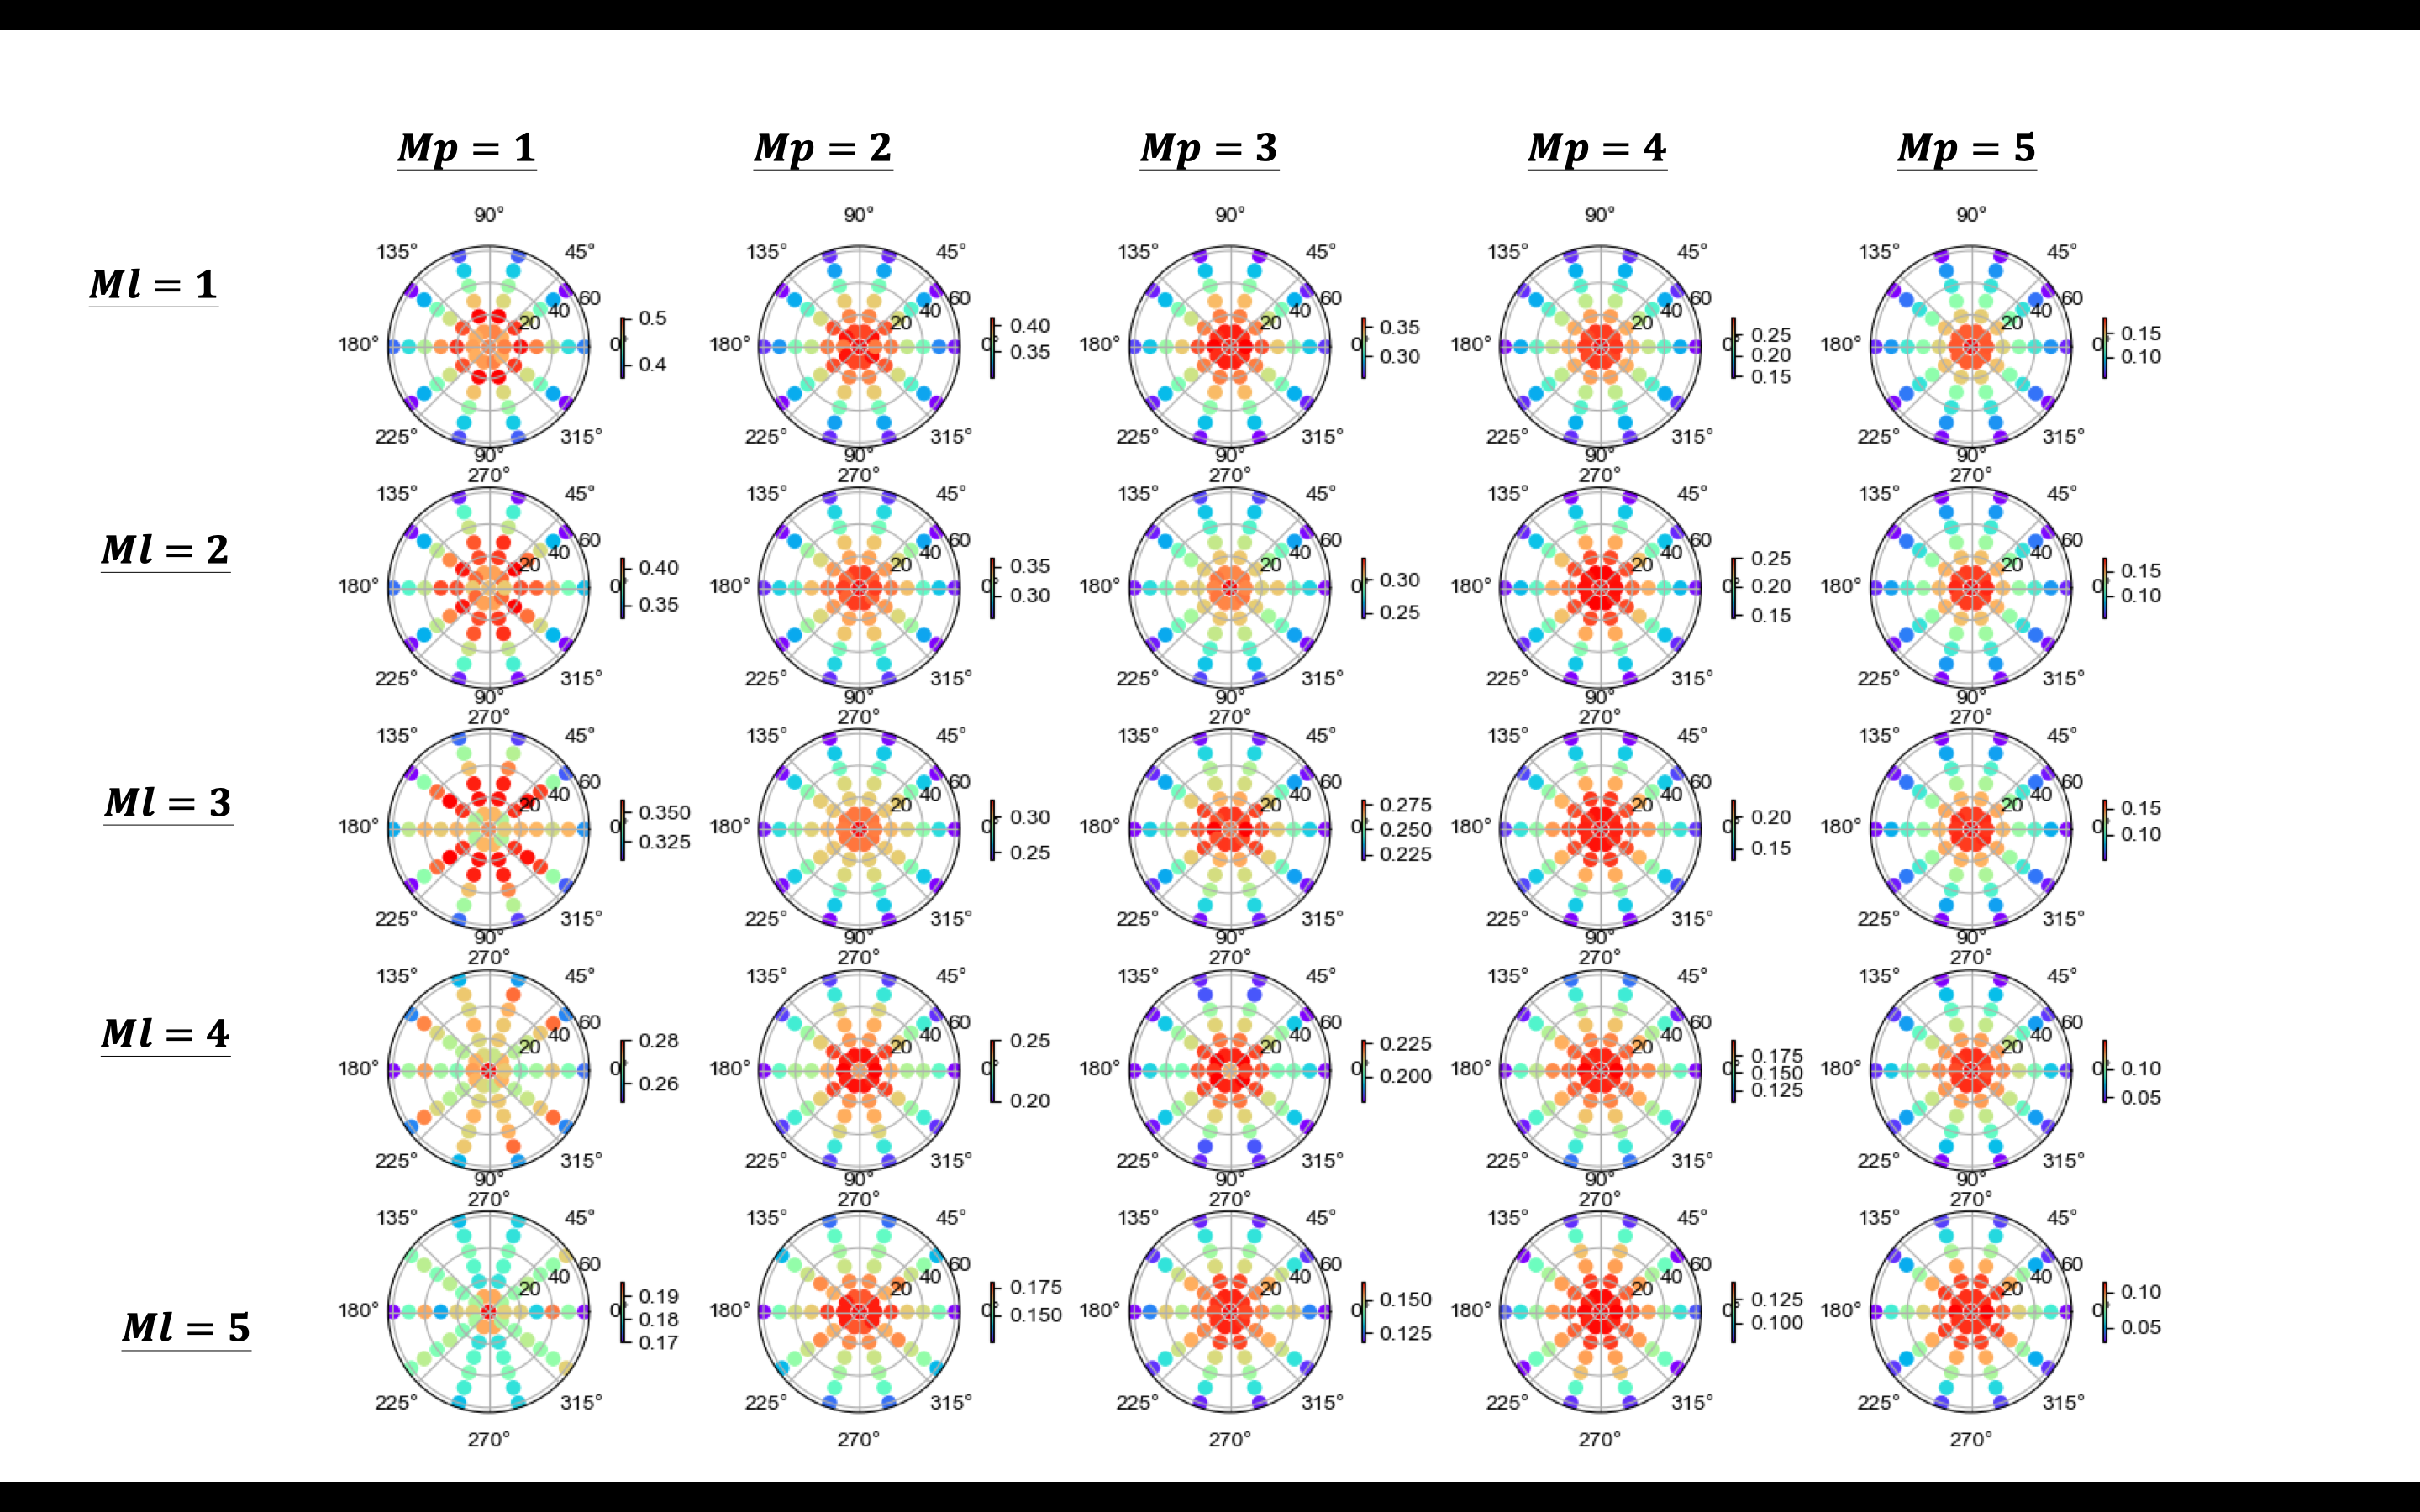
\includegraphics[width=14cm]{ch4pic/m_rotate.png}
%     \caption{改變硬體指向對旋轉樣本點的影響}
%     \label{pic:alpha_rotate}
% \end{figure}



\begin{figure}[htpb]
    \centering
    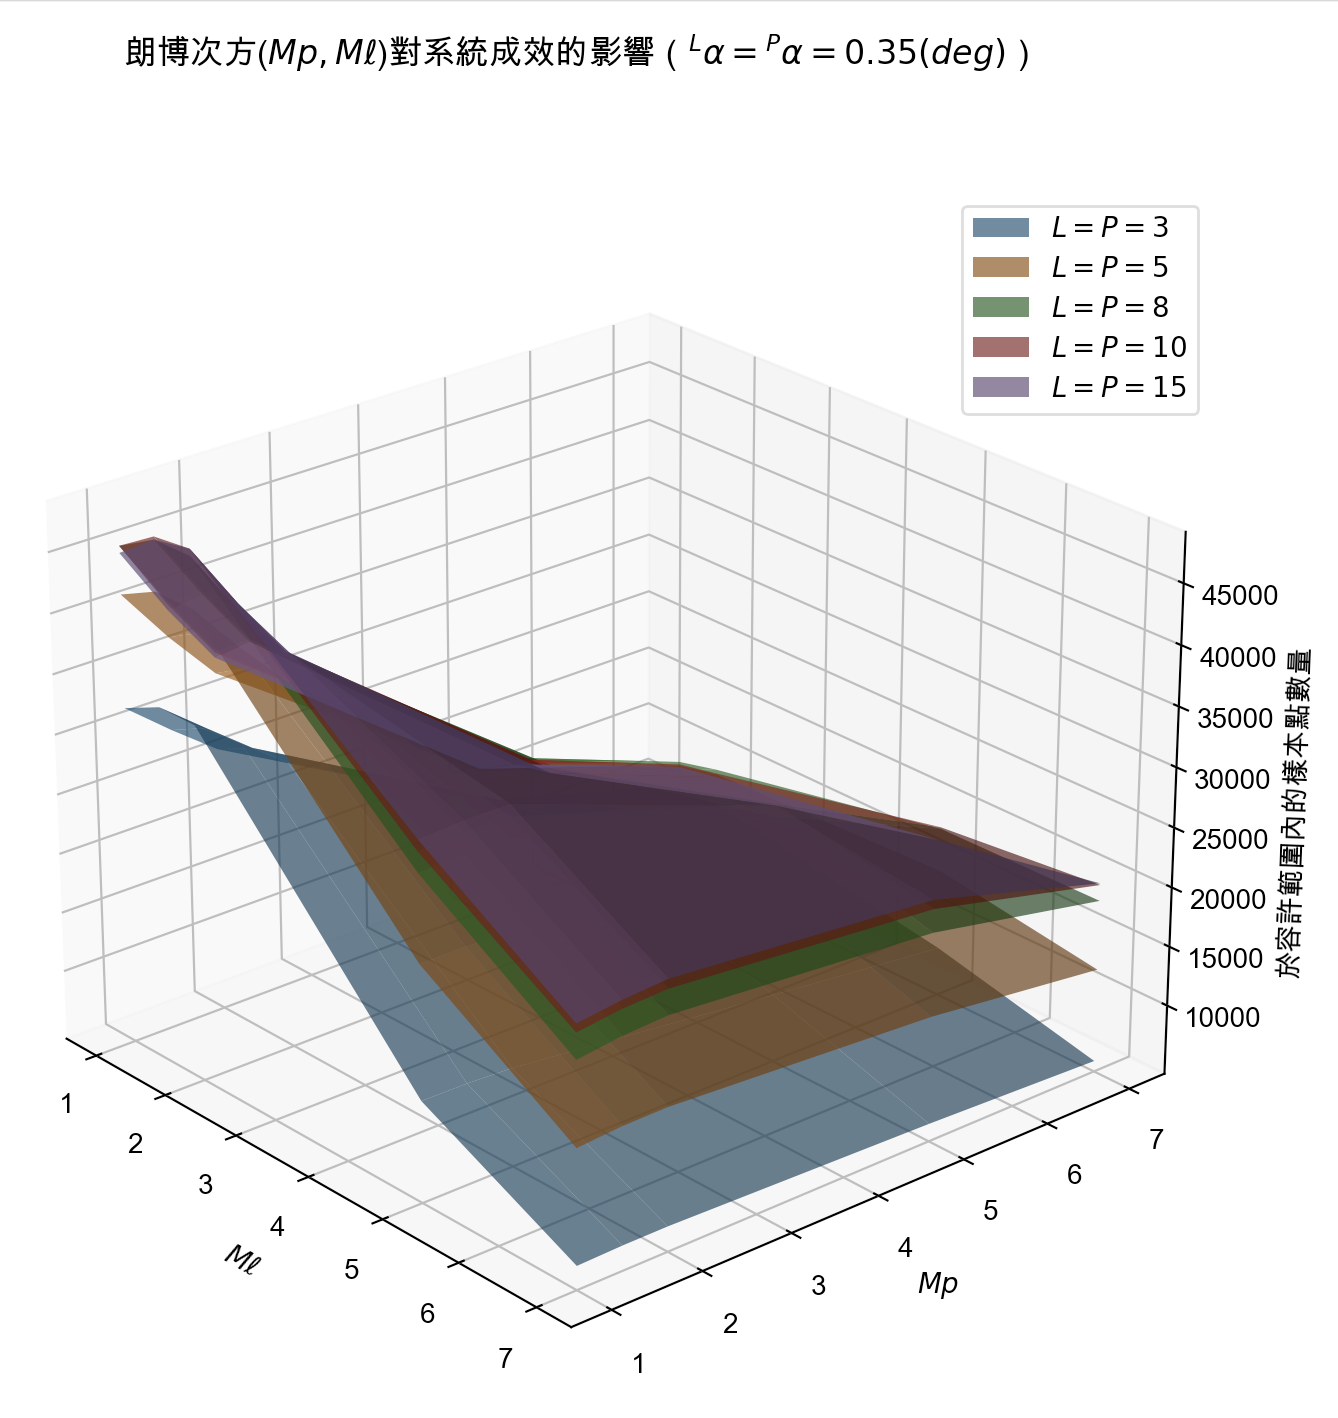
\includegraphics[width=9cm]{ch4pic/m_effect.png}
    \caption{改變硬體指向對系統的影響}
    \label{pic:alpha_effect}
\end{figure}



\subsubsection{硬體數量對系統表現的影響}
\label{chp:amount_effect}

由圖\ref{pic:m_effect}與圖\ref{pic:alpha_effect}中,我們都可以看出在提高硬體數量時,系統表現提升,然而系統表現提升的幅度不與硬體提升的數量成正比。因此,在挑選硬體數量時,除了系統表現以外,也需將硬體增加所造成的硬體成本,以及架設系統的難度考慮進來,在系統表現與硬體系統簡單中取捨。


% \subsection{不同使用情境的系統表現}


\section{結論}
\label{chp:4_conclusion}
由以上分析,我們可以看出在\ref{chp:scenario}章中提出的情境下,小的朗博次方與較小的硬體天頂角$\alpha$使系統的表現較佳,而硬體數量則是愈多愈好,但成長的趨勢隨著硬體數量增多而減慢。

我們本章節提出的方法,可以在軟體中透過改變硬體的選擇、樣本點的集合、組態等,快速的對不同情境,評估不同系統設計的表現。有了此模擬方法,我們可以在硬體系統架設之前對系統表現有所了解,避免在硬體架設的部分浪費時間與硬體成本。除此之外,藉由可以分析不同設計下的系統表現,我們進而於第五章針對不同情境,進行朗博次方、硬體指向以及硬體數量的最佳化,提供特定使用情境下的最佳系統設計。
%______________________________________



















% % --------------------------------------

















